\documentclass[twoside]{book}

% Packages required by doxygen
\usepackage{fixltx2e}
\usepackage{calc}
\usepackage{doxygen}
\usepackage[export]{adjustbox} % also loads graphicx
\usepackage{graphicx}
\usepackage[utf8]{inputenc}
\usepackage{makeidx}
\usepackage{multicol}
\usepackage{multirow}
\PassOptionsToPackage{warn}{textcomp}
\usepackage{textcomp}
\usepackage[nointegrals]{wasysym}
\usepackage[table]{xcolor}

% Font selection
\usepackage[T1]{fontenc}
\usepackage[scaled=.90]{helvet}
\usepackage{courier}
\usepackage{amssymb}
\usepackage{sectsty}
\renewcommand{\familydefault}{\sfdefault}
\allsectionsfont{%
  \fontseries{bc}\selectfont%
  \color{darkgray}%
}
\renewcommand{\DoxyLabelFont}{%
  \fontseries{bc}\selectfont%
  \color{darkgray}%
}
\newcommand{\+}{\discretionary{\mbox{\scriptsize$\hookleftarrow$}}{}{}}

% Page & text layout
\usepackage{geometry}
\geometry{%
  a4paper,%
  top=2.5cm,%
  bottom=2.5cm,%
  left=2.5cm,%
  right=2.5cm%
}
\tolerance=750
\hfuzz=15pt
\hbadness=750
\setlength{\emergencystretch}{15pt}
\setlength{\parindent}{0cm}
\setlength{\parskip}{0.2cm}
\makeatletter
\renewcommand{\paragraph}{%
  \@startsection{paragraph}{4}{0ex}{-1.0ex}{1.0ex}{%
    \normalfont\normalsize\bfseries\SS@parafont%
  }%
}
\renewcommand{\subparagraph}{%
  \@startsection{subparagraph}{5}{0ex}{-1.0ex}{1.0ex}{%
    \normalfont\normalsize\bfseries\SS@subparafont%
  }%
}
\makeatother

% Headers & footers
\usepackage{fancyhdr}
\pagestyle{fancyplain}
\fancyhead[LE]{\fancyplain{}{\bfseries\thepage}}
\fancyhead[CE]{\fancyplain{}{}}
\fancyhead[RE]{\fancyplain{}{\bfseries\leftmark}}
\fancyhead[LO]{\fancyplain{}{\bfseries\rightmark}}
\fancyhead[CO]{\fancyplain{}{}}
\fancyhead[RO]{\fancyplain{}{\bfseries\thepage}}
\fancyfoot[LE]{\fancyplain{}{}}
\fancyfoot[CE]{\fancyplain{}{}}
\fancyfoot[RE]{\fancyplain{}{\bfseries\scriptsize Generated on Mon Jun 8 2015 16\+:16\+:50 for My Project by Doxygen }}
\fancyfoot[LO]{\fancyplain{}{\bfseries\scriptsize Generated on Mon Jun 8 2015 16\+:16\+:50 for My Project by Doxygen }}
\fancyfoot[CO]{\fancyplain{}{}}
\fancyfoot[RO]{\fancyplain{}{}}
\renewcommand{\footrulewidth}{0.4pt}
\renewcommand{\chaptermark}[1]{%
  \markboth{#1}{}%
}
\renewcommand{\sectionmark}[1]{%
  \markright{\thesection\ #1}%
}

% Indices & bibliography
\usepackage{natbib}
\usepackage[titles]{tocloft}
\setcounter{tocdepth}{3}
\setcounter{secnumdepth}{5}
\makeindex

% Hyperlinks (required, but should be loaded last)
\usepackage{ifpdf}
\ifpdf
  \usepackage[pdftex,pagebackref=true]{hyperref}
\else
  \usepackage[ps2pdf,pagebackref=true]{hyperref}
\fi
\hypersetup{%
  colorlinks=true,%
  linkcolor=blue,%
  citecolor=blue,%
  unicode%
}

% Custom commands
\newcommand{\clearemptydoublepage}{%
  \newpage{\pagestyle{empty}\cleardoublepage}%
}


%===== C O N T E N T S =====

\begin{document}

% Titlepage & ToC
\hypersetup{pageanchor=false,
             bookmarks=true,
             bookmarksnumbered=true,
             pdfencoding=unicode
            }
\pagenumbering{roman}
\begin{titlepage}
\vspace*{7cm}
\begin{center}%
{\Large My Project }\\
\vspace*{1cm}
{\large Generated by Doxygen 1.8.9.1}\\
\vspace*{0.5cm}
{\small Mon Jun 8 2015 16:16:50}\\
\end{center}
\end{titlepage}
\clearemptydoublepage
\tableofcontents
\clearemptydoublepage
\pagenumbering{arabic}
\hypersetup{pageanchor=true}

%--- Begin generated contents ---
\chapter{Hierarchical Index}
\section{Class Hierarchy}
This inheritance list is sorted roughly, but not completely, alphabetically\+:\begin{DoxyCompactList}
\item \contentsline{section}{Block\+Data}{\pageref{struct_block_data}}{}
\item \contentsline{section}{Block\+Spawn\+Point}{\pageref{struct_block_spawn_point}}{}
\item \contentsline{section}{Bullet\+Launch\+Data}{\pageref{struct_bullet_launch_data}}{}
\item \contentsline{section}{Command}{\pageref{struct_command}}{}
\item \contentsline{section}{Command\+Queue}{\pageref{class_command_queue}}{}
\item \contentsline{section}{State\+:\+:Context}{\pageref{struct_state_1_1_context}}{}
\item \contentsline{section}{Direction}{\pageref{struct_direction}}{}
\item Drawable\begin{DoxyCompactList}
\item \contentsline{section}{G\+U\+I\+:\+:Component}{\pageref{class_g_u_i_1_1_component}}{}
\begin{DoxyCompactList}
\item \contentsline{section}{G\+U\+I\+:\+:Button}{\pageref{class_g_u_i_1_1_button}}{}
\item \contentsline{section}{G\+U\+I\+:\+:Container}{\pageref{class_g_u_i_1_1_container}}{}
\item \contentsline{section}{G\+U\+I\+:\+:Label}{\pageref{class_g_u_i_1_1_label}}{}
\end{DoxyCompactList}
\item \contentsline{section}{Quadtree}{\pageref{class_quadtree}}{}
\item \contentsline{section}{Scene\+Node}{\pageref{class_scene_node}}{}
\begin{DoxyCompactList}
\item \contentsline{section}{Block}{\pageref{class_block}}{}
\item \contentsline{section}{Entity}{\pageref{class_entity}}{}
\begin{DoxyCompactList}
\item \contentsline{section}{Projectile}{\pageref{class_projectile}}{}
\item \contentsline{section}{Tank}{\pageref{class_tank}}{}
\end{DoxyCompactList}
\item \contentsline{section}{Sprite\+Node}{\pageref{class_sprite_node}}{}
\item \contentsline{section}{Text\+Node}{\pageref{class_text_node}}{}
\end{DoxyCompactList}
\end{DoxyCompactList}
\item \contentsline{section}{Enemy\+Spawn\+Point}{\pageref{struct_enemy_spawn_point}}{}
\item \contentsline{section}{Level\+Data}{\pageref{struct_level_data}}{}
\item Non\+Copyable\begin{DoxyCompactList}
\item \contentsline{section}{Application}{\pageref{class_application}}{}
\item \contentsline{section}{G\+U\+I\+:\+:Component}{\pageref{class_g_u_i_1_1_component}}{}
\item \contentsline{section}{Scene\+Node}{\pageref{class_scene_node}}{}
\item \contentsline{section}{State\+Stack}{\pageref{class_state_stack}}{}
\item \contentsline{section}{World}{\pageref{class_world}}{}
\end{DoxyCompactList}
\item \contentsline{section}{Player}{\pageref{class_player}}{}
\item \contentsline{section}{Projectile\+Data}{\pageref{struct_projectile_data}}{}
\item \contentsline{section}{Resource\+Holder$<$ Resource, Identifier $>$}{\pageref{class_resource_holder}}{}
\item \contentsline{section}{Resource\+Holder$<$ sf\+:\+:Font, Fonts\+:\+:I\+D $>$}{\pageref{class_resource_holder}}{}
\item \contentsline{section}{Resource\+Holder$<$ sf\+:\+:Texture, Textures\+:\+:I\+D $>$}{\pageref{class_resource_holder}}{}
\item \contentsline{section}{State}{\pageref{class_state}}{}
\begin{DoxyCompactList}
\item \contentsline{section}{Game\+Over\+State}{\pageref{class_game_over_state}}{}
\item \contentsline{section}{Game\+State}{\pageref{class_game_state}}{}
\item \contentsline{section}{Menu\+State}{\pageref{class_menu_state}}{}
\item \contentsline{section}{Pause\+State}{\pageref{class_pause_state}}{}
\item \contentsline{section}{Settings\+State}{\pageref{class_settings_state}}{}
\item \contentsline{section}{Title\+State}{\pageref{class_title_state}}{}
\end{DoxyCompactList}
\item \contentsline{section}{Tank\+Data}{\pageref{struct_tank_data}}{}
\item Transformable\begin{DoxyCompactList}
\item \contentsline{section}{G\+U\+I\+:\+:Component}{\pageref{class_g_u_i_1_1_component}}{}
\item \contentsline{section}{Scene\+Node}{\pageref{class_scene_node}}{}
\end{DoxyCompactList}
\end{DoxyCompactList}

\chapter{Class Index}
\section{Class List}
Here are the classes, structs, unions and interfaces with brief descriptions\+:\begin{DoxyCompactList}
\item\contentsline{section}{\hyperlink{class_application}{Application} }{\pageref{class_application}}{}
\item\contentsline{section}{\hyperlink{class_block}{Block} }{\pageref{class_block}}{}
\item\contentsline{section}{\hyperlink{struct_block_data}{Block\+Data} }{\pageref{struct_block_data}}{}
\item\contentsline{section}{\hyperlink{struct_block_spawn_point}{Block\+Spawn\+Point} }{\pageref{struct_block_spawn_point}}{}
\item\contentsline{section}{\hyperlink{struct_bullet_launch_data}{Bullet\+Launch\+Data} }{\pageref{struct_bullet_launch_data}}{}
\item\contentsline{section}{\hyperlink{class_g_u_i_1_1_button}{G\+U\+I\+::\+Button} }{\pageref{class_g_u_i_1_1_button}}{}
\item\contentsline{section}{\hyperlink{struct_command}{Command} }{\pageref{struct_command}}{}
\item\contentsline{section}{\hyperlink{class_command_queue}{Command\+Queue} }{\pageref{class_command_queue}}{}
\item\contentsline{section}{\hyperlink{class_g_u_i_1_1_component}{G\+U\+I\+::\+Component} }{\pageref{class_g_u_i_1_1_component}}{}
\item\contentsline{section}{\hyperlink{class_g_u_i_1_1_container}{G\+U\+I\+::\+Container} }{\pageref{class_g_u_i_1_1_container}}{}
\item\contentsline{section}{\hyperlink{struct_state_1_1_context}{State\+::\+Context} }{\pageref{struct_state_1_1_context}}{}
\item\contentsline{section}{\hyperlink{struct_direction}{Direction} }{\pageref{struct_direction}}{}
\item\contentsline{section}{\hyperlink{struct_enemy_spawn_point}{Enemy\+Spawn\+Point} }{\pageref{struct_enemy_spawn_point}}{}
\item\contentsline{section}{\hyperlink{class_entity}{Entity} }{\pageref{class_entity}}{}
\item\contentsline{section}{\hyperlink{class_game_over_state}{Game\+Over\+State} }{\pageref{class_game_over_state}}{}
\item\contentsline{section}{\hyperlink{class_game_state}{Game\+State} }{\pageref{class_game_state}}{}
\item\contentsline{section}{\hyperlink{class_g_u_i_1_1_label}{G\+U\+I\+::\+Label} }{\pageref{class_g_u_i_1_1_label}}{}
\item\contentsline{section}{\hyperlink{struct_level_data}{Level\+Data} }{\pageref{struct_level_data}}{}
\item\contentsline{section}{\hyperlink{class_menu_state}{Menu\+State} }{\pageref{class_menu_state}}{}
\item\contentsline{section}{\hyperlink{class_pause_state}{Pause\+State} }{\pageref{class_pause_state}}{}
\item\contentsline{section}{\hyperlink{class_player}{Player} }{\pageref{class_player}}{}
\item\contentsline{section}{\hyperlink{class_projectile}{Projectile} }{\pageref{class_projectile}}{}
\item\contentsline{section}{\hyperlink{struct_projectile_data}{Projectile\+Data} }{\pageref{struct_projectile_data}}{}
\item\contentsline{section}{\hyperlink{class_quadtree}{Quadtree} }{\pageref{class_quadtree}}{}
\item\contentsline{section}{\hyperlink{class_resource_holder}{Resource\+Holder$<$ Resource, Identifier $>$} }{\pageref{class_resource_holder}}{}
\item\contentsline{section}{\hyperlink{class_scene_node}{Scene\+Node} }{\pageref{class_scene_node}}{}
\item\contentsline{section}{\hyperlink{class_settings_state}{Settings\+State} }{\pageref{class_settings_state}}{}
\item\contentsline{section}{\hyperlink{class_sprite_node}{Sprite\+Node} }{\pageref{class_sprite_node}}{}
\item\contentsline{section}{\hyperlink{class_state}{State} }{\pageref{class_state}}{}
\item\contentsline{section}{\hyperlink{class_state_stack}{State\+Stack} }{\pageref{class_state_stack}}{}
\item\contentsline{section}{\hyperlink{class_tank}{Tank} }{\pageref{class_tank}}{}
\item\contentsline{section}{\hyperlink{struct_tank_data}{Tank\+Data} }{\pageref{struct_tank_data}}{}
\item\contentsline{section}{\hyperlink{class_text_node}{Text\+Node} }{\pageref{class_text_node}}{}
\item\contentsline{section}{\hyperlink{class_title_state}{Title\+State} }{\pageref{class_title_state}}{}
\item\contentsline{section}{\hyperlink{class_world}{World} }{\pageref{class_world}}{}
\end{DoxyCompactList}

\chapter{Class Documentation}
\hypertarget{class_application}{}\section{Application Class Reference}
\label{class_application}\index{Application@{Application}}
Inheritance diagram for Application\+:\begin{figure}[H]
\begin{center}
\leavevmode
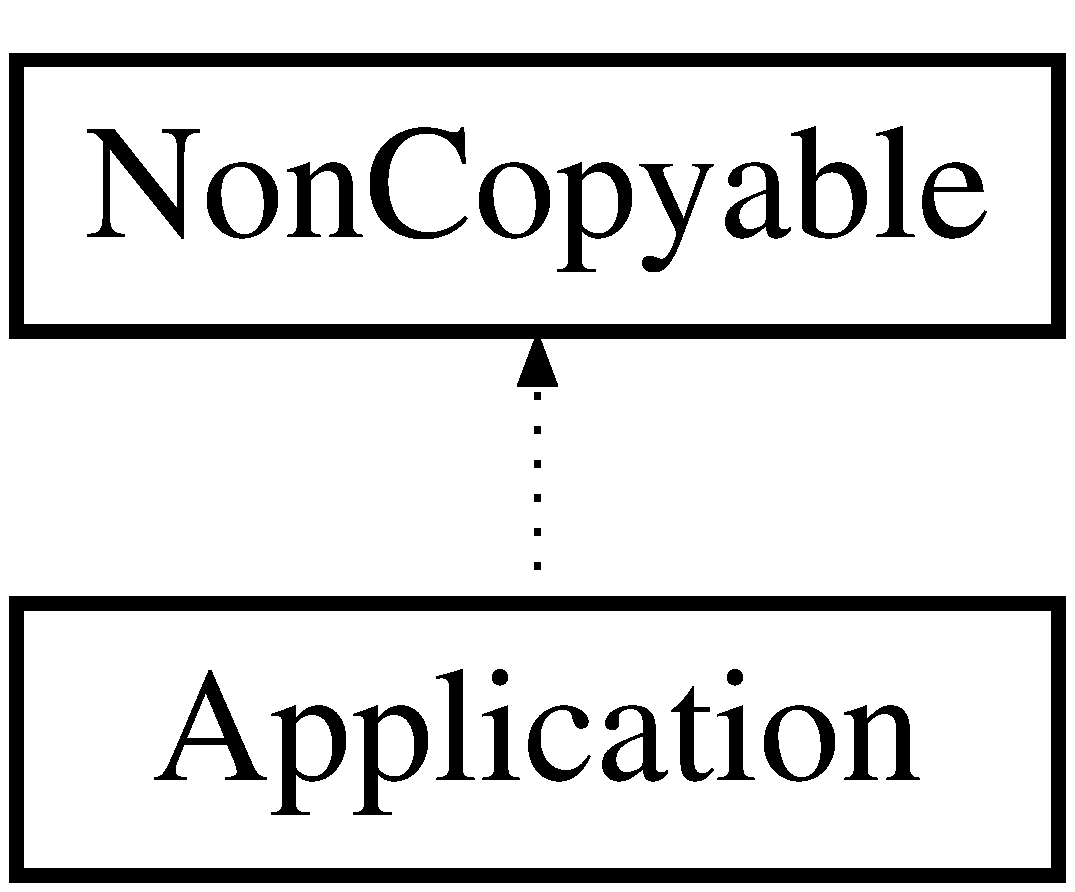
\includegraphics[height=2.000000cm]{class_application}
\end{center}
\end{figure}
\subsection*{Public Member Functions}
\begin{DoxyCompactItemize}
\item 
\hypertarget{class_application_a68965449404743bf1add056784d6cf81}{}void {\bfseries run} ()\label{class_application_a68965449404743bf1add056784d6cf81}

\end{DoxyCompactItemize}


The documentation for this class was generated from the following file\+:\begin{DoxyCompactItemize}
\item 
Include/\+Tanks/Application.\+hpp\end{DoxyCompactItemize}

\hypertarget{class_block}{}\section{Block Class Reference}
\label{class_block}\index{Block@{Block}}
Inheritance diagram for Block\+:\begin{figure}[H]
\begin{center}
\leavevmode
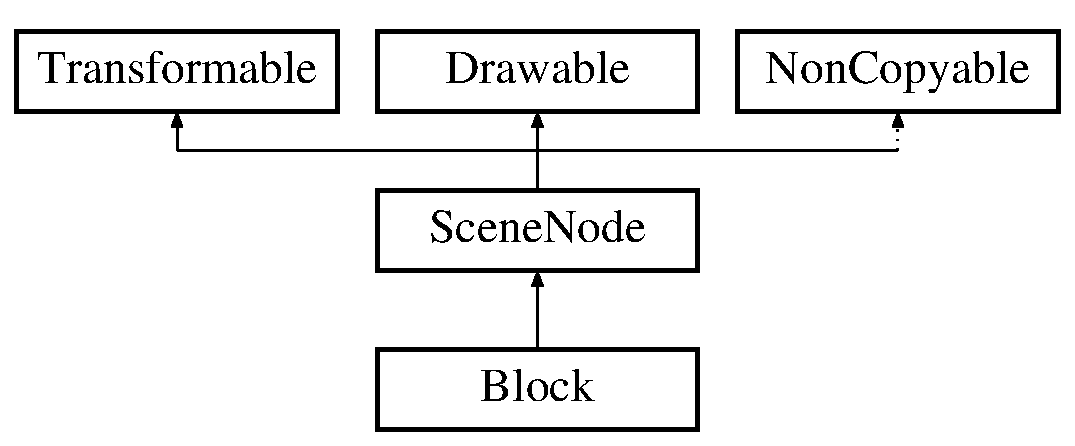
\includegraphics[height=3.000000cm]{class_block}
\end{center}
\end{figure}
\subsection*{Public Types}
\begin{DoxyCompactItemize}
\item 
\hypertarget{class_block_a2c6b3c425b9b8cb708b23e553fa81324}{}enum {\bfseries Type} \{ {\bfseries Indestructible}, 
{\bfseries Destructible}, 
{\bfseries Type\+Count}
 \}\label{class_block_a2c6b3c425b9b8cb708b23e553fa81324}

\end{DoxyCompactItemize}
\subsection*{Public Member Functions}
\begin{DoxyCompactItemize}
\item 
\hypertarget{class_block_a926042ca9b679390293daffe326b78ef}{}{\bfseries Block} (Block\+::\+Type type, sf\+::\+Vector2f size)\label{class_block_a926042ca9b679390293daffe326b78ef}

\item 
\hypertarget{class_block_a3a62a9c4a0e0ff093487cb44a5ed8fa5}{}virtual unsigned int {\bfseries get\+Category} () const \label{class_block_a3a62a9c4a0e0ff093487cb44a5ed8fa5}

\item 
\hypertarget{class_block_ae49c47399c54dfd923af82809f837643}{}virtual sf\+::\+Float\+Rect {\bfseries get\+Bounding\+Rect} () const \label{class_block_ae49c47399c54dfd923af82809f837643}

\item 
\hypertarget{class_block_ab719855e713ba62db29b1a211e12d94a}{}Type {\bfseries get\+Type} () const \label{class_block_ab719855e713ba62db29b1a211e12d94a}

\item 
\hypertarget{class_block_ab898d4e7d6a19056fe25f072a509cac8}{}sf\+::\+Vector2f {\bfseries get\+Size} () const \label{class_block_ab898d4e7d6a19056fe25f072a509cac8}

\item 
\hypertarget{class_block_abd587b2d58bc59094028828ba8fd15ab}{}void {\bfseries repair} (int points)\label{class_block_abd587b2d58bc59094028828ba8fd15ab}

\item 
\hypertarget{class_block_a81cad7086488a30c1cf87171a87708be}{}void {\bfseries damage} (int points)\label{class_block_a81cad7086488a30c1cf87171a87708be}

\item 
\hypertarget{class_block_a27b3bed5a1064d818cd61915f3a380bb}{}void {\bfseries destroy} ()\label{class_block_a27b3bed5a1064d818cd61915f3a380bb}

\item 
\hypertarget{class_block_ae046dec8383917e832d40309f8131075}{}int {\bfseries get\+Hitpoints} () const \label{class_block_ae046dec8383917e832d40309f8131075}

\item 
\hypertarget{class_block_a05fd29b6192dade0b2bf9636d89ef833}{}bool {\bfseries is\+Destroyed} () const \label{class_block_a05fd29b6192dade0b2bf9636d89ef833}

\end{DoxyCompactItemize}
\subsection*{Static Public Member Functions}
\begin{DoxyCompactItemize}
\item 
\hypertarget{class_block_ab49575e2c25a91b6a0edc7d620bf93a8}{}static int {\bfseries get\+Max\+Hitpoints} (Type type)\label{class_block_ab49575e2c25a91b6a0edc7d620bf93a8}

\end{DoxyCompactItemize}


The documentation for this class was generated from the following file\+:\begin{DoxyCompactItemize}
\item 
Include/\+Tanks/Block.\+hpp\end{DoxyCompactItemize}

\hypertarget{struct_block_data}{}\section{Block\+Data Struct Reference}
\label{struct_block_data}\index{Block\+Data@{Block\+Data}}
\subsection*{Public Attributes}
\begin{DoxyCompactItemize}
\item 
\hypertarget{struct_block_data_ab249be575a3ca36bea0a8ccbaae7555e}{}sf\+::\+Color {\bfseries color}\label{struct_block_data_ab249be575a3ca36bea0a8ccbaae7555e}

\item 
\hypertarget{struct_block_data_aaddfc6d873f27fab19c5034d0144fe00}{}int {\bfseries hitpoints}\label{struct_block_data_aaddfc6d873f27fab19c5034d0144fe00}

\end{DoxyCompactItemize}


The documentation for this struct was generated from the following file\+:\begin{DoxyCompactItemize}
\item 
Include/\+Tanks/Data\+Tables.\+hpp\end{DoxyCompactItemize}

\hypertarget{struct_block_spawn_point}{}\section{Block\+Spawn\+Point Struct Reference}
\label{struct_block_spawn_point}\index{Block\+Spawn\+Point@{Block\+Spawn\+Point}}
\subsection*{Public Member Functions}
\begin{DoxyCompactItemize}
\item 
\hypertarget{struct_block_spawn_point_a1f10b377017daf9e0ecbbab67ba9f4db}{}{\bfseries Block\+Spawn\+Point} (Block\+::\+Type type, float pos\+X, float pos\+Y, float size\+X, float size\+Y, int hitpoints)\label{struct_block_spawn_point_a1f10b377017daf9e0ecbbab67ba9f4db}

\end{DoxyCompactItemize}
\subsection*{Public Attributes}
\begin{DoxyCompactItemize}
\item 
\hypertarget{struct_block_spawn_point_a86b9ddbd98a8d16361407ff696a23e54}{}Block\+::\+Type {\bfseries type}\label{struct_block_spawn_point_a86b9ddbd98a8d16361407ff696a23e54}

\item 
\hypertarget{struct_block_spawn_point_acad0a5ad2123588f6f0fe0ba70e8151f}{}float {\bfseries pos\+X}\label{struct_block_spawn_point_acad0a5ad2123588f6f0fe0ba70e8151f}

\item 
\hypertarget{struct_block_spawn_point_a1828f6c8b339f389e51faee31748fb55}{}float {\bfseries pos\+Y}\label{struct_block_spawn_point_a1828f6c8b339f389e51faee31748fb55}

\item 
\hypertarget{struct_block_spawn_point_ab4f5e8ffb38404f07794538292a9d86c}{}float {\bfseries size\+X}\label{struct_block_spawn_point_ab4f5e8ffb38404f07794538292a9d86c}

\item 
\hypertarget{struct_block_spawn_point_aa8732ffb118fe2c3c855024bf7fda9b2}{}float {\bfseries size\+Y}\label{struct_block_spawn_point_aa8732ffb118fe2c3c855024bf7fda9b2}

\item 
\hypertarget{struct_block_spawn_point_a33b21c50009db97f4768da034292775e}{}int {\bfseries h}\label{struct_block_spawn_point_a33b21c50009db97f4768da034292775e}

\end{DoxyCompactItemize}


The documentation for this struct was generated from the following file\+:\begin{DoxyCompactItemize}
\item 
Include/\+Tanks/Spawn\+Point.\+hpp\end{DoxyCompactItemize}

\hypertarget{struct_bullet_launch_data}{}\section{Bullet\+Launch\+Data Struct Reference}
\label{struct_bullet_launch_data}\index{Bullet\+Launch\+Data@{Bullet\+Launch\+Data}}
\subsection*{Public Attributes}
\begin{DoxyCompactItemize}
\item 
\hypertarget{struct_bullet_launch_data_a65b9266464911ffaa47834f86b50041d}{}sf\+::\+Vector2f {\bfseries bullet\+Offset}\label{struct_bullet_launch_data_a65b9266464911ffaa47834f86b50041d}

\end{DoxyCompactItemize}


The documentation for this struct was generated from the following file\+:\begin{DoxyCompactItemize}
\item 
Include/\+Tanks/Data\+Tables.\+hpp\end{DoxyCompactItemize}

\hypertarget{class_g_u_i_1_1_button}{}\section{G\+U\+I\+:\+:Button Class Reference}
\label{class_g_u_i_1_1_button}\index{G\+U\+I\+::\+Button@{G\+U\+I\+::\+Button}}
Inheritance diagram for G\+U\+I\+:\+:Button\+:\begin{figure}[H]
\begin{center}
\leavevmode
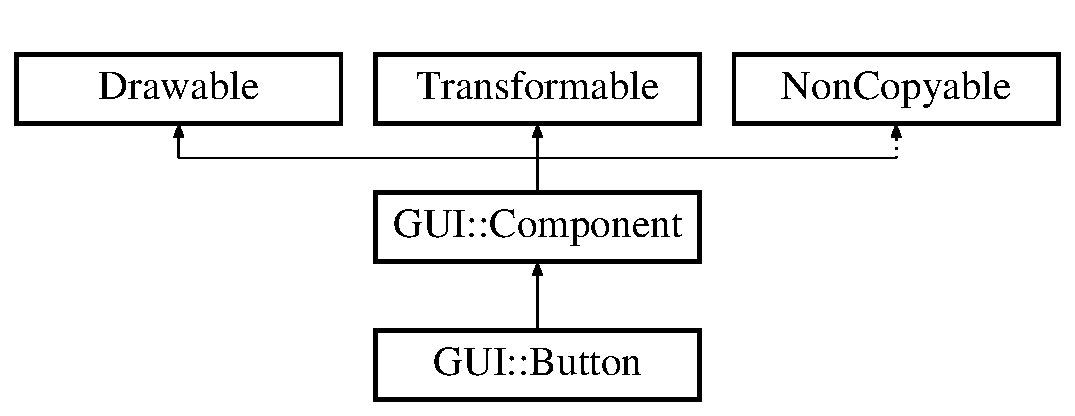
\includegraphics[height=3.000000cm]{class_g_u_i_1_1_button}
\end{center}
\end{figure}
\subsection*{Public Types}
\begin{DoxyCompactItemize}
\item 
\hypertarget{class_g_u_i_1_1_button_a910df9f7797f35d65b43da4dd392f1de}{}typedef std\+::shared\+\_\+ptr$<$ \hyperlink{class_g_u_i_1_1_button}{Button} $>$ {\bfseries Ptr}\label{class_g_u_i_1_1_button_a910df9f7797f35d65b43da4dd392f1de}

\item 
\hypertarget{class_g_u_i_1_1_button_a2d7e2cb4d20f8789a779a4133fe4c678}{}typedef std\+::function$<$ void()$>$ {\bfseries Callback}\label{class_g_u_i_1_1_button_a2d7e2cb4d20f8789a779a4133fe4c678}

\end{DoxyCompactItemize}
\subsection*{Public Member Functions}
\begin{DoxyCompactItemize}
\item 
\hypertarget{class_g_u_i_1_1_button_aa624162ff8bee4bd4523428c3ea2150b}{}{\bfseries Button} (const \hyperlink{class_resource_holder}{Font\+Holder} \&fonts, const \hyperlink{class_resource_holder}{Texture\+Holder} \&textures)\label{class_g_u_i_1_1_button_aa624162ff8bee4bd4523428c3ea2150b}

\item 
\hypertarget{class_g_u_i_1_1_button_ae5ac54c7429eaa482eb7069d0efdb79f}{}void {\bfseries set\+Callback} (Callback callback)\label{class_g_u_i_1_1_button_ae5ac54c7429eaa482eb7069d0efdb79f}

\item 
\hypertarget{class_g_u_i_1_1_button_a89e964d353192135d6a77aeff33bbc41}{}void {\bfseries set\+Text} (const std\+::string \&text)\label{class_g_u_i_1_1_button_a89e964d353192135d6a77aeff33bbc41}

\item 
\hypertarget{class_g_u_i_1_1_button_a8198052cf4fe5823c9f5513e778ca94d}{}void {\bfseries set\+Toggle} (bool flag)\label{class_g_u_i_1_1_button_a8198052cf4fe5823c9f5513e778ca94d}

\item 
\hypertarget{class_g_u_i_1_1_button_ab494980476e92b67878c8b86958e4768}{}virtual bool {\bfseries is\+Selectable} () const \label{class_g_u_i_1_1_button_ab494980476e92b67878c8b86958e4768}

\item 
\hypertarget{class_g_u_i_1_1_button_af18d9012525f9431bb86127d248e4851}{}virtual void {\bfseries select} ()\label{class_g_u_i_1_1_button_af18d9012525f9431bb86127d248e4851}

\item 
\hypertarget{class_g_u_i_1_1_button_a93596a77391e32c54da2b6699e08aaf3}{}virtual void {\bfseries deselect} ()\label{class_g_u_i_1_1_button_a93596a77391e32c54da2b6699e08aaf3}

\item 
\hypertarget{class_g_u_i_1_1_button_adb322ef2c0bf27c9a28e22464732859b}{}virtual void {\bfseries activate} ()\label{class_g_u_i_1_1_button_adb322ef2c0bf27c9a28e22464732859b}

\item 
\hypertarget{class_g_u_i_1_1_button_a02c8762837eb47fe1965f75d4580a59b}{}virtual void {\bfseries deactivate} ()\label{class_g_u_i_1_1_button_a02c8762837eb47fe1965f75d4580a59b}

\item 
\hypertarget{class_g_u_i_1_1_button_ab015659c2c765a0dbf3a7201a60726cd}{}virtual void {\bfseries handle\+Event} (const sf\+::\+Event \&event)\label{class_g_u_i_1_1_button_ab015659c2c765a0dbf3a7201a60726cd}

\end{DoxyCompactItemize}


The documentation for this class was generated from the following file\+:\begin{DoxyCompactItemize}
\item 
Include/\+Tanks/Button.\+hpp\end{DoxyCompactItemize}

\hypertarget{struct_command}{}\section{Command Struct Reference}
\label{struct_command}\index{Command@{Command}}
\subsection*{Public Attributes}
\begin{DoxyCompactItemize}
\item 
\hypertarget{struct_command_a104fe6a9eb7bc8fc2f23acc67eb2b1d9}{}std\+::function$<$ void(\hyperlink{class_scene_node}{Scene\+Node} \&, sf\+::\+Time)$>$ {\bfseries action}\label{struct_command_a104fe6a9eb7bc8fc2f23acc67eb2b1d9}

\item 
\hypertarget{struct_command_a1529e898c9e6dd47b1826b5b1eac09fb}{}unsigned int {\bfseries category}\label{struct_command_a1529e898c9e6dd47b1826b5b1eac09fb}

\end{DoxyCompactItemize}


The documentation for this struct was generated from the following file\+:\begin{DoxyCompactItemize}
\item 
Include/\+Tanks/Command.\+hpp\end{DoxyCompactItemize}

\hypertarget{class_command_queue}{}\section{Command\+Queue Class Reference}
\label{class_command_queue}\index{Command\+Queue@{Command\+Queue}}
\subsection*{Public Member Functions}
\begin{DoxyCompactItemize}
\item 
\hypertarget{class_command_queue_ad444e0d7af45d9e09b834f0cec1e1f43}{}void {\bfseries push} (const \hyperlink{struct_command}{Command} \&command)\label{class_command_queue_ad444e0d7af45d9e09b834f0cec1e1f43}

\item 
\hypertarget{class_command_queue_ac2dde510222b8df393b55978f4594194}{}\hyperlink{struct_command}{Command} {\bfseries pop} ()\label{class_command_queue_ac2dde510222b8df393b55978f4594194}

\item 
\hypertarget{class_command_queue_ad4f4731c185a293724a59aba9a5903d6}{}bool {\bfseries is\+Empty} () const \label{class_command_queue_ad4f4731c185a293724a59aba9a5903d6}

\end{DoxyCompactItemize}


The documentation for this class was generated from the following file\+:\begin{DoxyCompactItemize}
\item 
Include/\+Tanks/Command\+Queue.\+hpp\end{DoxyCompactItemize}

\hypertarget{class_g_u_i_1_1_component}{}\section{G\+U\+I\+:\+:Component Class Reference}
\label{class_g_u_i_1_1_component}\index{G\+U\+I\+::\+Component@{G\+U\+I\+::\+Component}}
Inheritance diagram for G\+U\+I\+:\+:Component\+:\begin{figure}[H]
\begin{center}
\leavevmode
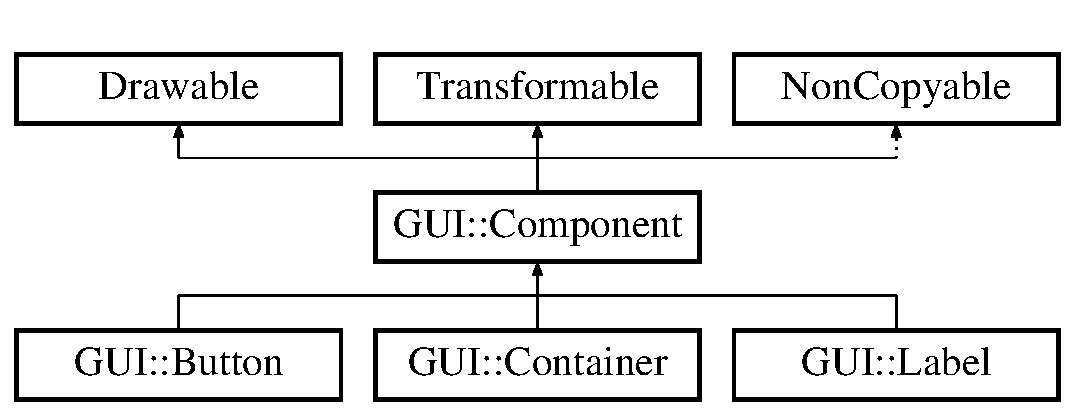
\includegraphics[height=3.000000cm]{class_g_u_i_1_1_component}
\end{center}
\end{figure}
\subsection*{Public Types}
\begin{DoxyCompactItemize}
\item 
\hypertarget{class_g_u_i_1_1_component_aa51eb17541f4cbe71b60cf7e1e16f32b}{}typedef std\+::shared\+\_\+ptr$<$ \hyperlink{class_g_u_i_1_1_component}{Component} $>$ {\bfseries Ptr}\label{class_g_u_i_1_1_component_aa51eb17541f4cbe71b60cf7e1e16f32b}

\end{DoxyCompactItemize}
\subsection*{Public Member Functions}
\begin{DoxyCompactItemize}
\item 
\hypertarget{class_g_u_i_1_1_component_a44d14506c9a1dbc839e05a6bf99c341b}{}virtual bool {\bfseries is\+Selectable} () const =0\label{class_g_u_i_1_1_component_a44d14506c9a1dbc839e05a6bf99c341b}

\item 
\hypertarget{class_g_u_i_1_1_component_affb93ae274f3dd3f44da70520d13b07d}{}bool {\bfseries is\+Selected} () const \label{class_g_u_i_1_1_component_affb93ae274f3dd3f44da70520d13b07d}

\item 
\hypertarget{class_g_u_i_1_1_component_ae807056061554da9c0e99b380eb9e480}{}virtual void {\bfseries select} ()\label{class_g_u_i_1_1_component_ae807056061554da9c0e99b380eb9e480}

\item 
\hypertarget{class_g_u_i_1_1_component_acd7bf93ec3553fdbdfadc8402ee967df}{}virtual void {\bfseries deselect} ()\label{class_g_u_i_1_1_component_acd7bf93ec3553fdbdfadc8402ee967df}

\item 
\hypertarget{class_g_u_i_1_1_component_a7b750c7c3f9b9910ac775b969116e001}{}virtual bool {\bfseries is\+Active} () const \label{class_g_u_i_1_1_component_a7b750c7c3f9b9910ac775b969116e001}

\item 
\hypertarget{class_g_u_i_1_1_component_a6c2bfb067dc3bfa9dc833cd3e6cba807}{}virtual void {\bfseries activate} ()\label{class_g_u_i_1_1_component_a6c2bfb067dc3bfa9dc833cd3e6cba807}

\item 
\hypertarget{class_g_u_i_1_1_component_adca7b246109fa739ebcd608637746364}{}virtual void {\bfseries deactivate} ()\label{class_g_u_i_1_1_component_adca7b246109fa739ebcd608637746364}

\item 
\hypertarget{class_g_u_i_1_1_component_aacf5e981e7b5726f5c7e9436455660ba}{}virtual void {\bfseries handle\+Event} (const sf\+::\+Event \&event)=0\label{class_g_u_i_1_1_component_aacf5e981e7b5726f5c7e9436455660ba}

\end{DoxyCompactItemize}


The documentation for this class was generated from the following file\+:\begin{DoxyCompactItemize}
\item 
Include/\+Tanks/Component.\+hpp\end{DoxyCompactItemize}

\hypertarget{class_g_u_i_1_1_container}{}\section{G\+U\+I\+:\+:Container Class Reference}
\label{class_g_u_i_1_1_container}\index{G\+U\+I\+::\+Container@{G\+U\+I\+::\+Container}}
Inheritance diagram for G\+U\+I\+:\+:Container\+:\begin{figure}[H]
\begin{center}
\leavevmode
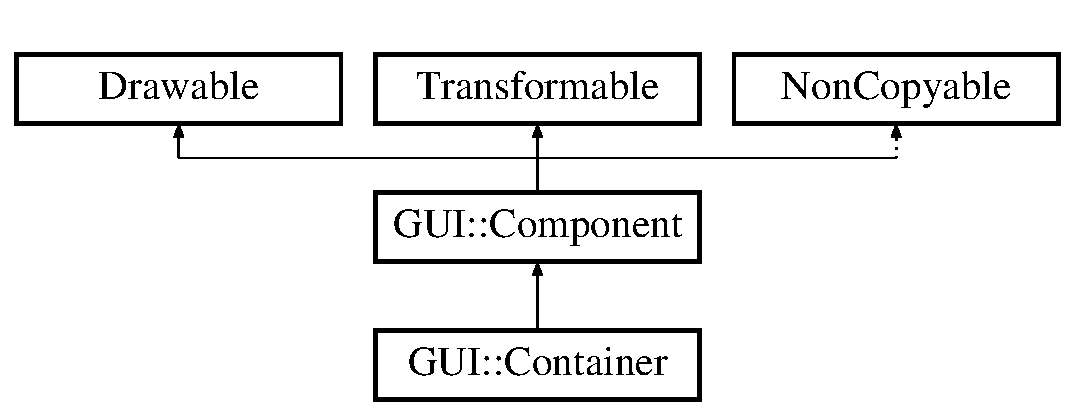
\includegraphics[height=3.000000cm]{class_g_u_i_1_1_container}
\end{center}
\end{figure}
\subsection*{Public Types}
\begin{DoxyCompactItemize}
\item 
\hypertarget{class_g_u_i_1_1_container_aff900329cc0dbef99abdd1c95175823a}{}typedef std\+::shared\+\_\+ptr$<$ \hyperlink{class_g_u_i_1_1_container}{Container} $>$ {\bfseries Ptr}\label{class_g_u_i_1_1_container_aff900329cc0dbef99abdd1c95175823a}

\end{DoxyCompactItemize}
\subsection*{Public Member Functions}
\begin{DoxyCompactItemize}
\item 
\hypertarget{class_g_u_i_1_1_container_a96138fff70a580a2c0184347be95c74c}{}void {\bfseries pack} (Component\+::\+Ptr component)\label{class_g_u_i_1_1_container_a96138fff70a580a2c0184347be95c74c}

\item 
\hypertarget{class_g_u_i_1_1_container_aacc4f2be899907bd6b03e28dd229fac2}{}virtual bool {\bfseries is\+Selectable} () const \label{class_g_u_i_1_1_container_aacc4f2be899907bd6b03e28dd229fac2}

\item 
\hypertarget{class_g_u_i_1_1_container_adc3b4318b7cb683482f0d0de5b1431d3}{}virtual void {\bfseries handle\+Event} (const sf\+::\+Event \&event)\label{class_g_u_i_1_1_container_adc3b4318b7cb683482f0d0de5b1431d3}

\end{DoxyCompactItemize}


The documentation for this class was generated from the following file\+:\begin{DoxyCompactItemize}
\item 
Include/\+Tanks/Container.\+hpp\end{DoxyCompactItemize}

\hypertarget{struct_state_1_1_context}{}\section{State\+:\+:Context Struct Reference}
\label{struct_state_1_1_context}\index{State\+::\+Context@{State\+::\+Context}}
\subsection*{Public Member Functions}
\begin{DoxyCompactItemize}
\item 
\hypertarget{struct_state_1_1_context_ac8380f7873b3248c7cf32c604bbdda26}{}{\bfseries Context} (sf\+::\+Render\+Window \&window, \hyperlink{class_resource_holder}{Texture\+Holder} \&textures, \hyperlink{class_resource_holder}{Font\+Holder} \&fonts, \hyperlink{class_player}{Player} \&player)\label{struct_state_1_1_context_ac8380f7873b3248c7cf32c604bbdda26}

\end{DoxyCompactItemize}
\subsection*{Public Attributes}
\begin{DoxyCompactItemize}
\item 
\hypertarget{struct_state_1_1_context_a30775e70e841c761a4e3cb7f0e195128}{}sf\+::\+Render\+Window $\ast$ {\bfseries window}\label{struct_state_1_1_context_a30775e70e841c761a4e3cb7f0e195128}

\item 
\hypertarget{struct_state_1_1_context_a587123ee3b00e8c68c1d99ca6011a53d}{}\hyperlink{class_resource_holder}{Texture\+Holder} $\ast$ {\bfseries textures}\label{struct_state_1_1_context_a587123ee3b00e8c68c1d99ca6011a53d}

\item 
\hypertarget{struct_state_1_1_context_a8b4a94c250018312ccf2e58a33f0c77a}{}\hyperlink{class_resource_holder}{Font\+Holder} $\ast$ {\bfseries fonts}\label{struct_state_1_1_context_a8b4a94c250018312ccf2e58a33f0c77a}

\item 
\hypertarget{struct_state_1_1_context_a1c98434687748acdebf78fd80a4767ad}{}\hyperlink{class_player}{Player} $\ast$ {\bfseries player}\label{struct_state_1_1_context_a1c98434687748acdebf78fd80a4767ad}

\end{DoxyCompactItemize}


The documentation for this struct was generated from the following file\+:\begin{DoxyCompactItemize}
\item 
Include/\+Tanks/State.\+hpp\end{DoxyCompactItemize}

\hypertarget{struct_direction}{}\section{Direction Struct Reference}
\label{struct_direction}\index{Direction@{Direction}}
\subsection*{Public Member Functions}
\begin{DoxyCompactItemize}
\item 
\hypertarget{struct_direction_a4b7fbea88026265cf268369987ec4bb7}{}{\bfseries Direction} (float movement\+Angle, float distance, float rotation)\label{struct_direction_a4b7fbea88026265cf268369987ec4bb7}

\end{DoxyCompactItemize}
\subsection*{Public Attributes}
\begin{DoxyCompactItemize}
\item 
\hypertarget{struct_direction_a8eaabd2d06c6274e92866814cfb6a2ea}{}float {\bfseries angle}\label{struct_direction_a8eaabd2d06c6274e92866814cfb6a2ea}

\item 
\hypertarget{struct_direction_a6cf81244bffe43d4b4d1bc8a3f63772a}{}float {\bfseries distance}\label{struct_direction_a6cf81244bffe43d4b4d1bc8a3f63772a}

\item 
\hypertarget{struct_direction_adc976fea5f08991089819266d9acbca5}{}float {\bfseries rotation}\label{struct_direction_adc976fea5f08991089819266d9acbca5}

\end{DoxyCompactItemize}


The documentation for this struct was generated from the following file\+:\begin{DoxyCompactItemize}
\item 
Include/\+Tanks/Direction.\+hpp\end{DoxyCompactItemize}

\hypertarget{struct_enemy_spawn_point}{}\section{Enemy\+Spawn\+Point Struct Reference}
\label{struct_enemy_spawn_point}\index{Enemy\+Spawn\+Point@{Enemy\+Spawn\+Point}}
\subsection*{Public Member Functions}
\begin{DoxyCompactItemize}
\item 
\hypertarget{struct_enemy_spawn_point_afd541169e2d2c338a37b36e5db701dde}{}{\bfseries Enemy\+Spawn\+Point} (Tank\+::\+Type type, float x, float y, float rotation, int number\+Of\+Kills, int hitpoints, float guarding\+Path\+Length=0.f, float guarding\+Angle=0.f, float travelled\+Distance=0.f, float amount\+Rotation=0.f, std\+::size\+\_\+t direction\+Index=0)\label{struct_enemy_spawn_point_afd541169e2d2c338a37b36e5db701dde}

\end{DoxyCompactItemize}
\subsection*{Public Attributes}
\begin{DoxyCompactItemize}
\item 
\hypertarget{struct_enemy_spawn_point_af4a2702c7808b9dd4002a8cd67119603}{}Tank\+::\+Type {\bfseries type}\label{struct_enemy_spawn_point_af4a2702c7808b9dd4002a8cd67119603}

\item 
\hypertarget{struct_enemy_spawn_point_a6b9ff06f1aa09043e675105f3e302d43}{}float {\bfseries x}\label{struct_enemy_spawn_point_a6b9ff06f1aa09043e675105f3e302d43}

\item 
\hypertarget{struct_enemy_spawn_point_a3301e2687a721f82d5e1cd60b56806d0}{}float {\bfseries y}\label{struct_enemy_spawn_point_a3301e2687a721f82d5e1cd60b56806d0}

\item 
\hypertarget{struct_enemy_spawn_point_a222bed8d5d664432c31cc3c133c754cf}{}float {\bfseries r}\label{struct_enemy_spawn_point_a222bed8d5d664432c31cc3c133c754cf}

\item 
\hypertarget{struct_enemy_spawn_point_aa6db28a2d501639d39179be2d0e944b8}{}int {\bfseries n}\label{struct_enemy_spawn_point_aa6db28a2d501639d39179be2d0e944b8}

\item 
\hypertarget{struct_enemy_spawn_point_a57a2d3a947c7f20774a5589e91aae030}{}int {\bfseries h}\label{struct_enemy_spawn_point_a57a2d3a947c7f20774a5589e91aae030}

\item 
\hypertarget{struct_enemy_spawn_point_a34055eac45cc2ca2cbb72034f972da61}{}float {\bfseries gpl}\label{struct_enemy_spawn_point_a34055eac45cc2ca2cbb72034f972da61}

\item 
\hypertarget{struct_enemy_spawn_point_aafaa8262fb403e40da8bb75518e627d8}{}float {\bfseries ga}\label{struct_enemy_spawn_point_aafaa8262fb403e40da8bb75518e627d8}

\item 
\hypertarget{struct_enemy_spawn_point_ad51b53e12ecd480a90b3750337c300a7}{}float {\bfseries td}\label{struct_enemy_spawn_point_ad51b53e12ecd480a90b3750337c300a7}

\item 
\hypertarget{struct_enemy_spawn_point_a3459088a7b10307fd1b165f6e007895a}{}float {\bfseries ar}\label{struct_enemy_spawn_point_a3459088a7b10307fd1b165f6e007895a}

\item 
\hypertarget{struct_enemy_spawn_point_a0cf5d8de51f554a3bd1644bba054d60e}{}std\+::size\+\_\+t {\bfseries di}\label{struct_enemy_spawn_point_a0cf5d8de51f554a3bd1644bba054d60e}

\end{DoxyCompactItemize}


The documentation for this struct was generated from the following file\+:\begin{DoxyCompactItemize}
\item 
Include/\+Tanks/Spawn\+Point.\+hpp\end{DoxyCompactItemize}

\hypertarget{class_entity}{}\section{Entity Class Reference}
\label{class_entity}\index{Entity@{Entity}}
Inheritance diagram for Entity\+:\begin{figure}[H]
\begin{center}
\leavevmode
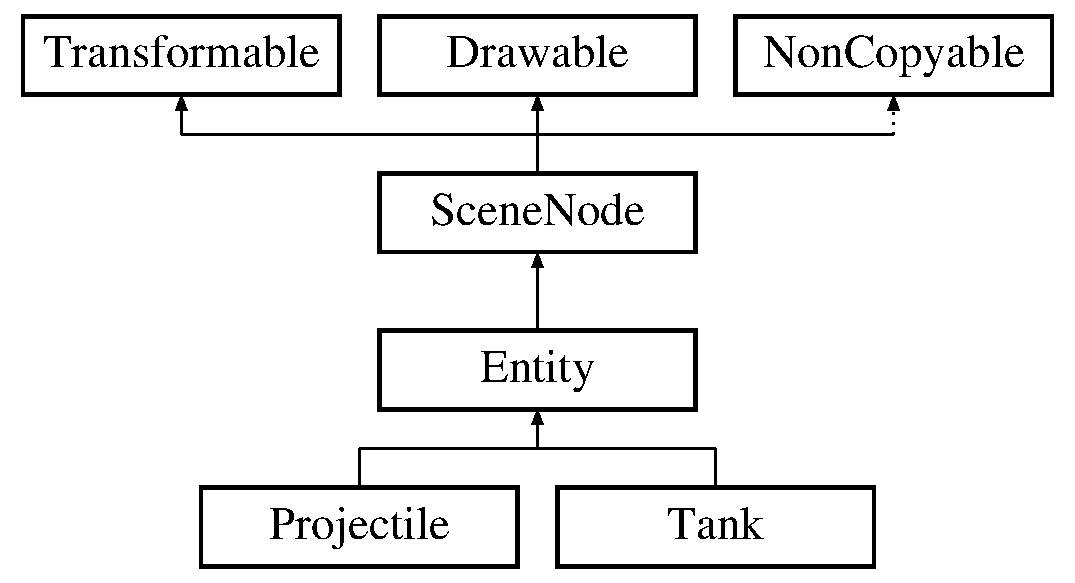
\includegraphics[height=4.000000cm]{class_entity}
\end{center}
\end{figure}
\subsection*{Public Member Functions}
\begin{DoxyCompactItemize}
\item 
\hypertarget{class_entity_a305ac3dd729c288ab23db531fa3fb7e6}{}{\bfseries Entity} (int hitpoints)\label{class_entity_a305ac3dd729c288ab23db531fa3fb7e6}

\item 
\hypertarget{class_entity_a5bf79843c973eac1fdbebfd1fc83a1e8}{}void {\bfseries set\+Velocity} (sf\+::\+Vector2f velocity)\label{class_entity_a5bf79843c973eac1fdbebfd1fc83a1e8}

\item 
\hypertarget{class_entity_a7873fbd61cf1a742d4492ec438a9ac9f}{}void {\bfseries set\+Velocity} (float vx, float vy)\label{class_entity_a7873fbd61cf1a742d4492ec438a9ac9f}

\item 
\hypertarget{class_entity_a80cdb89f11d47716781bc567efd2bcda}{}void {\bfseries accelerate} (sf\+::\+Vector2f velocity)\label{class_entity_a80cdb89f11d47716781bc567efd2bcda}

\item 
\hypertarget{class_entity_a2ff2403c455f15b3fe5d04e922b3943d}{}void {\bfseries accelerate} (float vx, float vy)\label{class_entity_a2ff2403c455f15b3fe5d04e922b3943d}

\item 
\hypertarget{class_entity_ad428181660f03f4a800461e1810e5937}{}sf\+::\+Vector2f {\bfseries get\+Velocity} () const \label{class_entity_ad428181660f03f4a800461e1810e5937}

\item 
\hypertarget{class_entity_a354ea9f771b0758f8e70bdfac9a740b4}{}void {\bfseries repair} (int points)\label{class_entity_a354ea9f771b0758f8e70bdfac9a740b4}

\item 
\hypertarget{class_entity_a15660fa13012dbca80c8047e2cc6f1f5}{}void {\bfseries damage} (int points)\label{class_entity_a15660fa13012dbca80c8047e2cc6f1f5}

\item 
\hypertarget{class_entity_a691dbe5f9ec930c27af2af0b97907a9e}{}void {\bfseries destroy} ()\label{class_entity_a691dbe5f9ec930c27af2af0b97907a9e}

\item 
\hypertarget{class_entity_a23125d6943b71a3d9a43d5271262a654}{}int {\bfseries get\+Hitpoints} () const \label{class_entity_a23125d6943b71a3d9a43d5271262a654}

\item 
\hypertarget{class_entity_a3c86039d4c16de3490b52a8595440f47}{}bool {\bfseries is\+Destroyed} () const \label{class_entity_a3c86039d4c16de3490b52a8595440f47}

\end{DoxyCompactItemize}
\subsection*{Protected Member Functions}
\begin{DoxyCompactItemize}
\item 
\hypertarget{class_entity_a4ebebbbb20fcac7024fb3a9985ed2eff}{}virtual void {\bfseries update\+Current} (sf\+::\+Time dt, \hyperlink{class_command_queue}{Command\+Queue} \&commands)\label{class_entity_a4ebebbbb20fcac7024fb3a9985ed2eff}

\end{DoxyCompactItemize}
\subsection*{Additional Inherited Members}


The documentation for this class was generated from the following file\+:\begin{DoxyCompactItemize}
\item 
Include/\+Tanks/Entity.\+hpp\end{DoxyCompactItemize}

\hypertarget{class_game_over_state}{}\section{Game\+Over\+State Class Reference}
\label{class_game_over_state}\index{Game\+Over\+State@{Game\+Over\+State}}
Inheritance diagram for Game\+Over\+State\+:\begin{figure}[H]
\begin{center}
\leavevmode
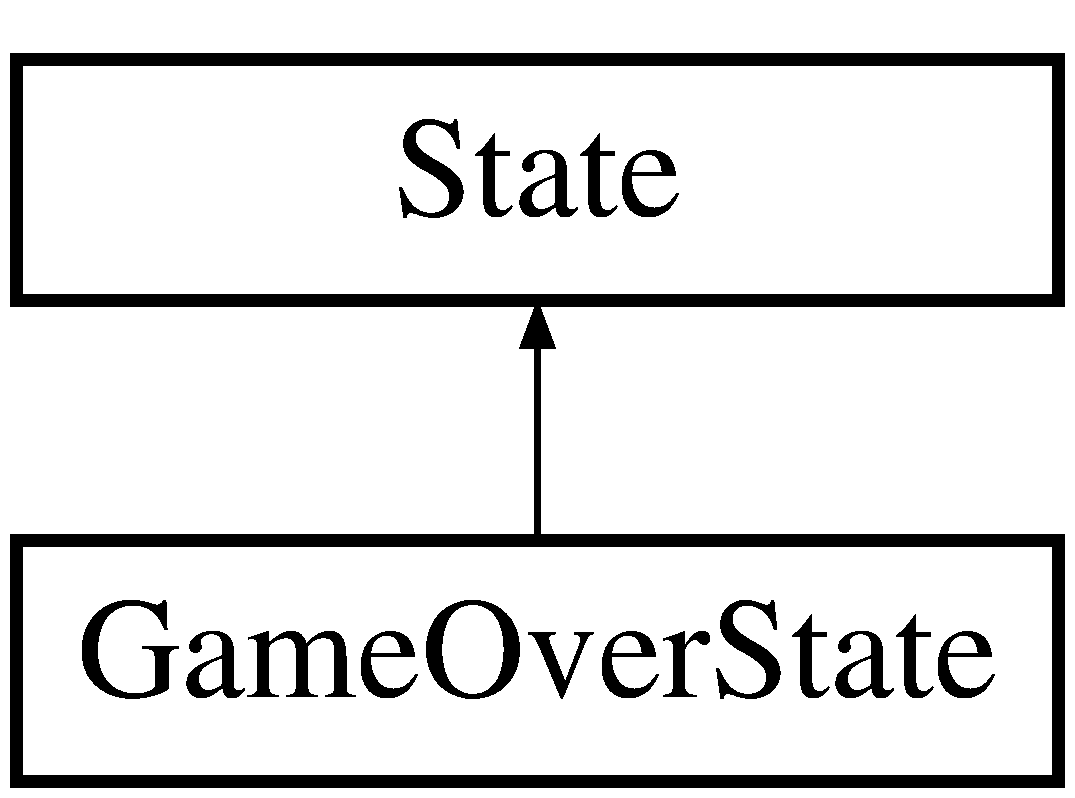
\includegraphics[height=2.000000cm]{class_game_over_state}
\end{center}
\end{figure}
\subsection*{Public Member Functions}
\begin{DoxyCompactItemize}
\item 
\hypertarget{class_game_over_state_a45b48ddc81da6e2afa0ef647fd83a123}{}{\bfseries Game\+Over\+State} (\hyperlink{class_state_stack}{State\+Stack} \&stack, \hyperlink{struct_state_1_1_context}{Context} context)\label{class_game_over_state_a45b48ddc81da6e2afa0ef647fd83a123}

\item 
\hypertarget{class_game_over_state_ae2d0593d5344c719bf33fcbb31feee9e}{}virtual void {\bfseries draw} ()\label{class_game_over_state_ae2d0593d5344c719bf33fcbb31feee9e}

\item 
\hypertarget{class_game_over_state_a83adaa9e20dee01b9ca855542532e0cf}{}virtual bool {\bfseries update} (sf\+::\+Time dt)\label{class_game_over_state_a83adaa9e20dee01b9ca855542532e0cf}

\item 
\hypertarget{class_game_over_state_a55ff5cbeb9960405bd9e433fd1f897b8}{}virtual bool {\bfseries handle\+Event} (const sf\+::\+Event \&event)\label{class_game_over_state_a55ff5cbeb9960405bd9e433fd1f897b8}

\end{DoxyCompactItemize}
\subsection*{Additional Inherited Members}


The documentation for this class was generated from the following file\+:\begin{DoxyCompactItemize}
\item 
Include/\+Tanks/Game\+Over\+State.\+hpp\end{DoxyCompactItemize}

\hypertarget{class_game_state}{}\section{Game\+State Class Reference}
\label{class_game_state}\index{Game\+State@{Game\+State}}
Inheritance diagram for Game\+State\+:\begin{figure}[H]
\begin{center}
\leavevmode
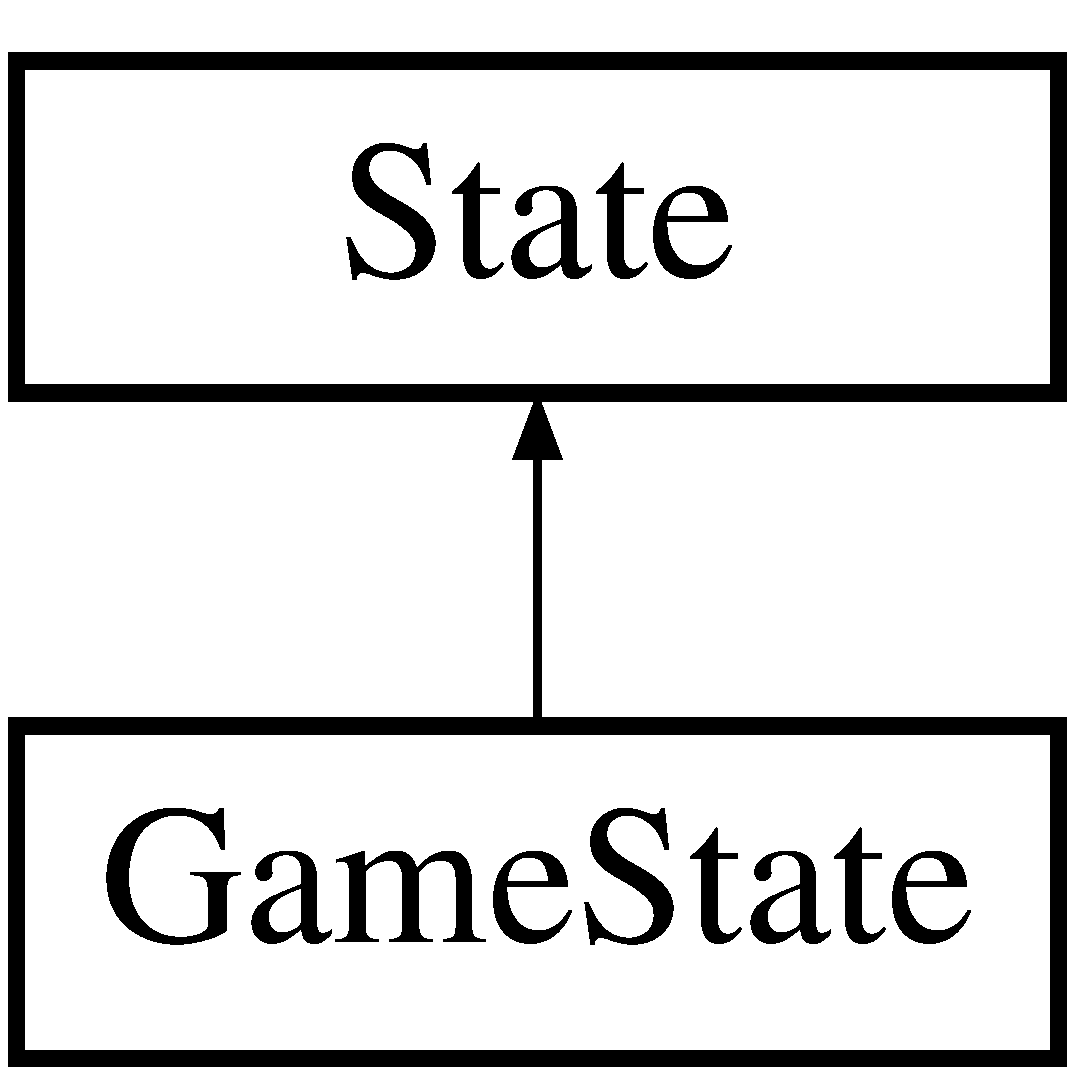
\includegraphics[height=2.000000cm]{class_game_state}
\end{center}
\end{figure}
\subsection*{Public Member Functions}
\begin{DoxyCompactItemize}
\item 
\hypertarget{class_game_state_aeb2e2598754640c694b989311b1aebfe}{}{\bfseries Game\+State} (\hyperlink{class_state_stack}{State\+Stack} \&stack, \hyperlink{struct_state_1_1_context}{Context} context)\label{class_game_state_aeb2e2598754640c694b989311b1aebfe}

\item 
\hypertarget{class_game_state_adf753ecc90e0b309c849b117036e619e}{}virtual void {\bfseries draw} ()\label{class_game_state_adf753ecc90e0b309c849b117036e619e}

\item 
\hypertarget{class_game_state_a0b13d7c27239f0cfc7260955a960d045}{}virtual bool {\bfseries update} (sf\+::\+Time dt)\label{class_game_state_a0b13d7c27239f0cfc7260955a960d045}

\item 
\hypertarget{class_game_state_a063c526c647305d7bac9ae95b3f9078f}{}virtual bool {\bfseries handle\+Event} (const sf\+::\+Event \&event)\label{class_game_state_a063c526c647305d7bac9ae95b3f9078f}

\end{DoxyCompactItemize}
\subsection*{Additional Inherited Members}


The documentation for this class was generated from the following file\+:\begin{DoxyCompactItemize}
\item 
Include/\+Tanks/Game\+State.\+hpp\end{DoxyCompactItemize}

\hypertarget{class_g_u_i_1_1_label}{}\section{G\+U\+I\+:\+:Label Class Reference}
\label{class_g_u_i_1_1_label}\index{G\+U\+I\+::\+Label@{G\+U\+I\+::\+Label}}
Inheritance diagram for G\+U\+I\+:\+:Label\+:\begin{figure}[H]
\begin{center}
\leavevmode
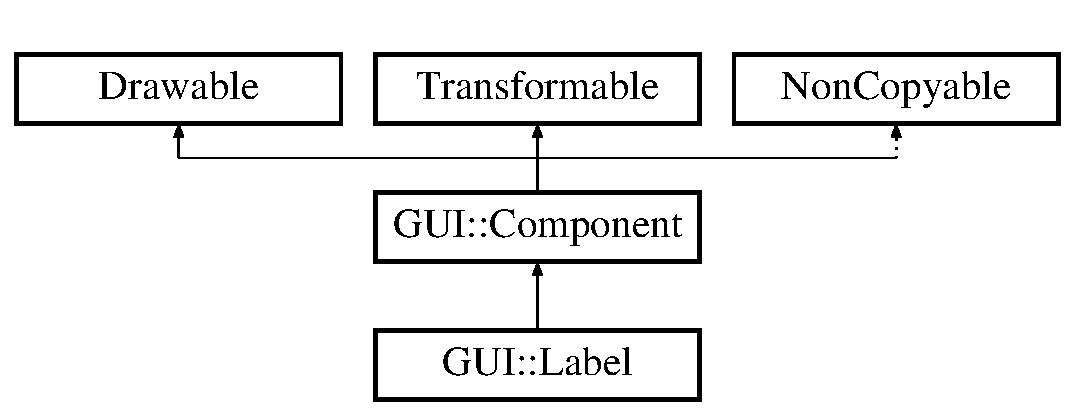
\includegraphics[height=3.000000cm]{class_g_u_i_1_1_label}
\end{center}
\end{figure}
\subsection*{Public Types}
\begin{DoxyCompactItemize}
\item 
\hypertarget{class_g_u_i_1_1_label_aa00f786f8578a677ef7b979aa28c2546}{}typedef std\+::shared\+\_\+ptr$<$ \hyperlink{class_g_u_i_1_1_label}{Label} $>$ {\bfseries Ptr}\label{class_g_u_i_1_1_label_aa00f786f8578a677ef7b979aa28c2546}

\end{DoxyCompactItemize}
\subsection*{Public Member Functions}
\begin{DoxyCompactItemize}
\item 
\hypertarget{class_g_u_i_1_1_label_af7776f7b27736bf53a41b8aec79a60c5}{}{\bfseries Label} (const std\+::string \&text, const \hyperlink{class_resource_holder}{Font\+Holder} \&fonts)\label{class_g_u_i_1_1_label_af7776f7b27736bf53a41b8aec79a60c5}

\item 
\hypertarget{class_g_u_i_1_1_label_afa6abd1c4f2bb812e8fdf426be4c90fa}{}virtual bool {\bfseries is\+Selectable} () const \label{class_g_u_i_1_1_label_afa6abd1c4f2bb812e8fdf426be4c90fa}

\item 
\hypertarget{class_g_u_i_1_1_label_ab86467acdbe18a9fda4712a177e16dae}{}void {\bfseries set\+Text} (const std\+::string \&text)\label{class_g_u_i_1_1_label_ab86467acdbe18a9fda4712a177e16dae}

\item 
\hypertarget{class_g_u_i_1_1_label_a69d78318d537190aebbba1ab07363367}{}virtual void {\bfseries handle\+Event} (const sf\+::\+Event \&event)\label{class_g_u_i_1_1_label_a69d78318d537190aebbba1ab07363367}

\end{DoxyCompactItemize}


The documentation for this class was generated from the following file\+:\begin{DoxyCompactItemize}
\item 
Include/\+Tanks/Label.\+hpp\end{DoxyCompactItemize}

\hypertarget{struct_level_data}{}\section{Level\+Data Struct Reference}
\label{struct_level_data}\index{Level\+Data@{Level\+Data}}
\subsection*{Public Attributes}
\begin{DoxyCompactItemize}
\item 
\hypertarget{struct_level_data_a406ab5513d875228b1cef9bfe445ed65}{}Textures\+::\+I\+D {\bfseries background\+Texture}\label{struct_level_data_a406ab5513d875228b1cef9bfe445ed65}

\item 
\hypertarget{struct_level_data_a255b0e592f1e66b66f155e6574bc3978}{}World\+::\+View\+Type {\bfseries view\+Type}\label{struct_level_data_a255b0e592f1e66b66f155e6574bc3978}

\item 
\hypertarget{struct_level_data_a19d1bba4aa13d1e0e73a3b2b5f67ad0b}{}sf\+::\+Float\+Rect {\bfseries world\+Bounds}\label{struct_level_data_a19d1bba4aa13d1e0e73a3b2b5f67ad0b}

\item 
\hypertarget{struct_level_data_a458576f1378738a57d6bb75d6bc975f4}{}sf\+::\+Vector2f {\bfseries player\+Spawn\+Position}\label{struct_level_data_a458576f1378738a57d6bb75d6bc975f4}

\item 
\hypertarget{struct_level_data_ad4a2359abca4b03d93dfd4115e909620}{}std\+::vector$<$ \hyperlink{struct_enemy_spawn_point}{Enemy\+Spawn\+Point} $>$ {\bfseries enemy\+Spawn\+Points}\label{struct_level_data_ad4a2359abca4b03d93dfd4115e909620}

\item 
\hypertarget{struct_level_data_a200661b03076406a0648f45bcf6d5d44}{}std\+::vector$<$ \hyperlink{struct_block_spawn_point}{Block\+Spawn\+Point} $>$ {\bfseries block\+Spawn\+Points}\label{struct_level_data_a200661b03076406a0648f45bcf6d5d44}

\end{DoxyCompactItemize}


The documentation for this struct was generated from the following file\+:\begin{DoxyCompactItemize}
\item 
Include/\+Tanks/Data\+Tables.\+hpp\end{DoxyCompactItemize}

\hypertarget{class_menu_state}{}\section{Menu\+State Class Reference}
\label{class_menu_state}\index{Menu\+State@{Menu\+State}}
Inheritance diagram for Menu\+State\+:\begin{figure}[H]
\begin{center}
\leavevmode
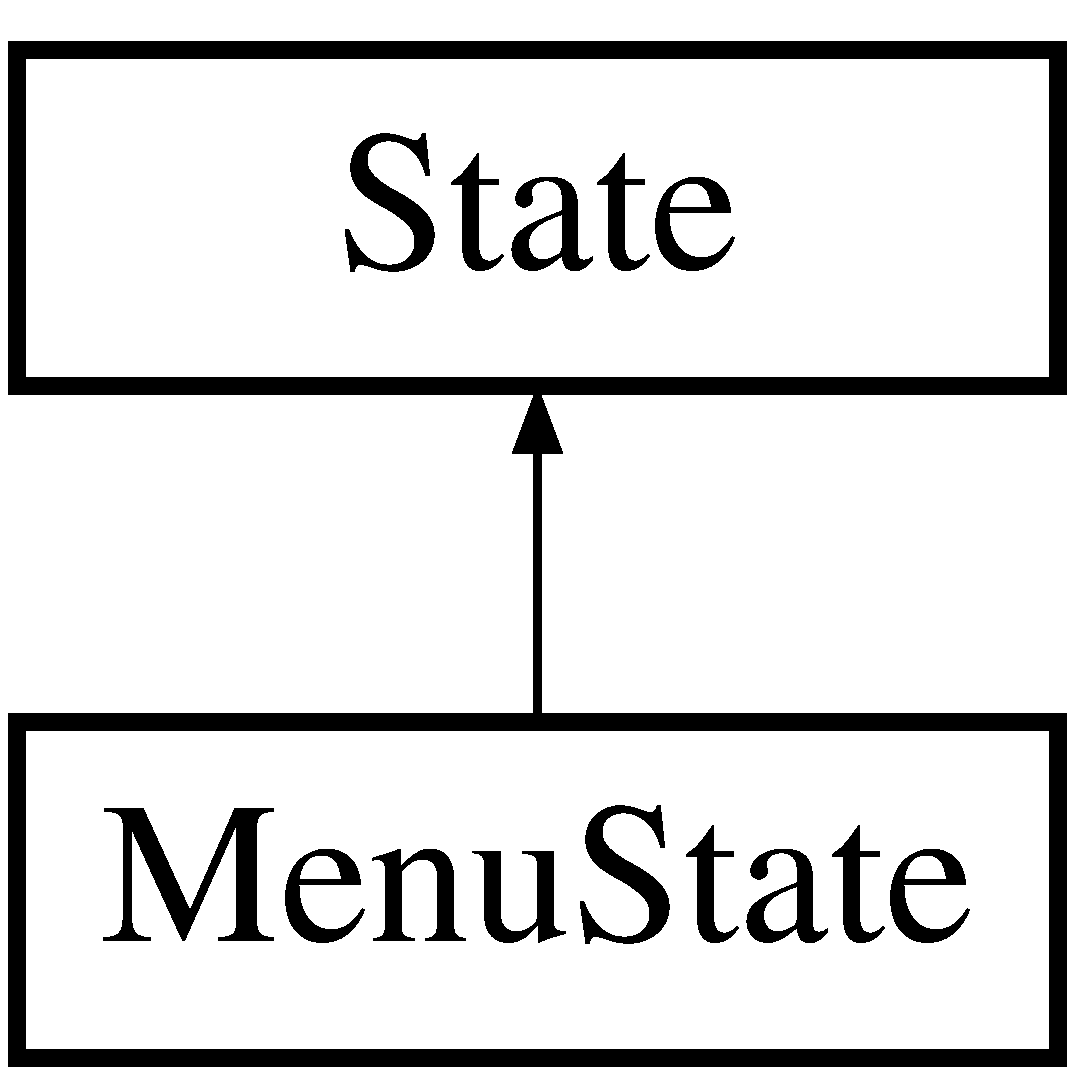
\includegraphics[height=2.000000cm]{class_menu_state}
\end{center}
\end{figure}
\subsection*{Public Member Functions}
\begin{DoxyCompactItemize}
\item 
\hypertarget{class_menu_state_a6e7034c57bf83f24aa8f4321d3d210a5}{}{\bfseries Menu\+State} (\hyperlink{class_state_stack}{State\+Stack} \&stack, \hyperlink{struct_state_1_1_context}{Context} context)\label{class_menu_state_a6e7034c57bf83f24aa8f4321d3d210a5}

\item 
\hypertarget{class_menu_state_a7214f8d8b7ecd282100d1ca1a1dc168f}{}virtual void {\bfseries draw} ()\label{class_menu_state_a7214f8d8b7ecd282100d1ca1a1dc168f}

\item 
\hypertarget{class_menu_state_a588a73443b2eca91edc895fe5a2a94ce}{}virtual bool {\bfseries update} (sf\+::\+Time dt)\label{class_menu_state_a588a73443b2eca91edc895fe5a2a94ce}

\item 
\hypertarget{class_menu_state_a985853550bfe9569b2e446f1b9ecb5af}{}virtual bool {\bfseries handle\+Event} (const sf\+::\+Event \&event)\label{class_menu_state_a985853550bfe9569b2e446f1b9ecb5af}

\end{DoxyCompactItemize}
\subsection*{Additional Inherited Members}


The documentation for this class was generated from the following file\+:\begin{DoxyCompactItemize}
\item 
Include/\+Tanks/Menu\+State.\+hpp\end{DoxyCompactItemize}

\hypertarget{class_pause_state}{}\section{Pause\+State Class Reference}
\label{class_pause_state}\index{Pause\+State@{Pause\+State}}
Inheritance diagram for Pause\+State\+:\begin{figure}[H]
\begin{center}
\leavevmode
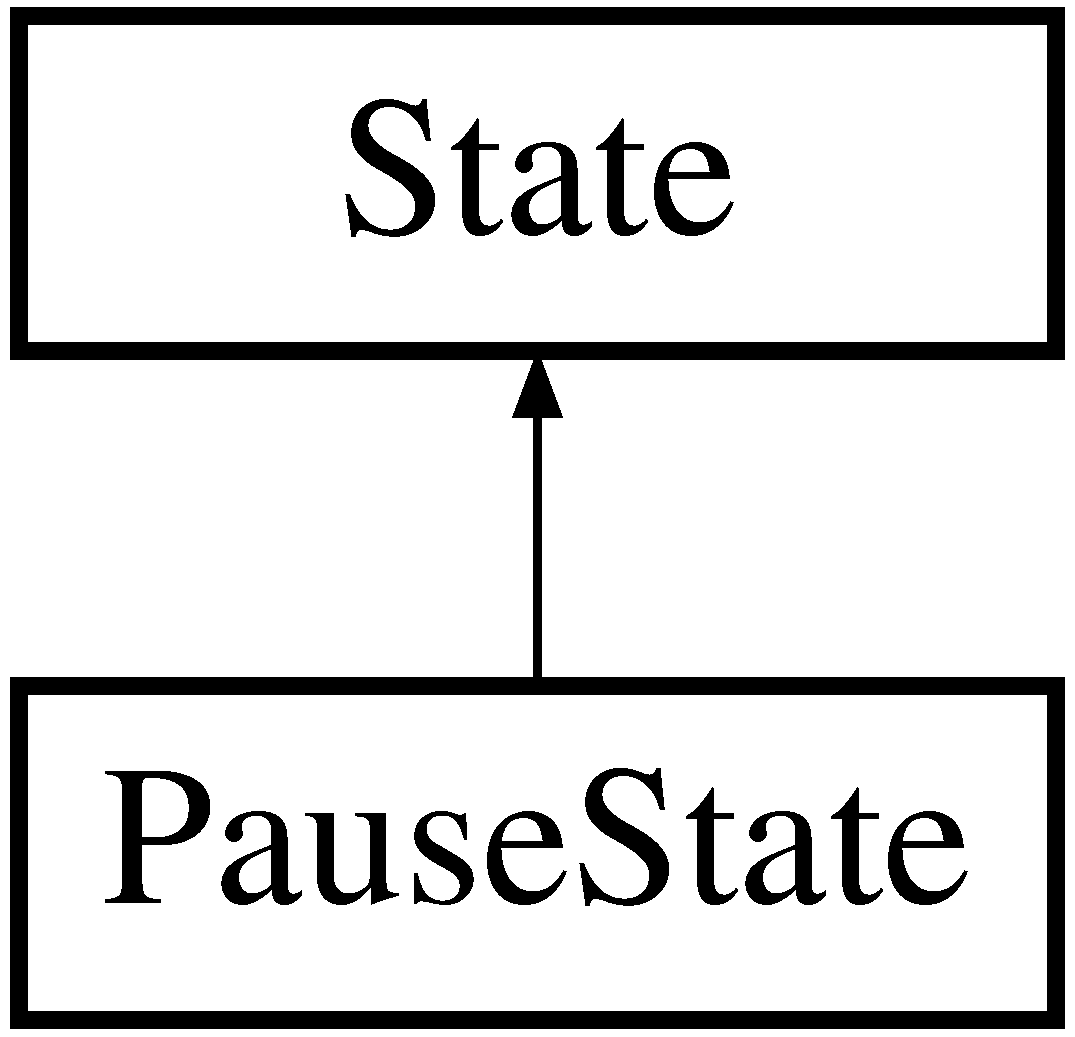
\includegraphics[height=2.000000cm]{class_pause_state}
\end{center}
\end{figure}
\subsection*{Public Member Functions}
\begin{DoxyCompactItemize}
\item 
\hypertarget{class_pause_state_ac5c14226e18f688233f5b511e1025a59}{}{\bfseries Pause\+State} (\hyperlink{class_state_stack}{State\+Stack} \&stack, \hyperlink{struct_state_1_1_context}{Context} context)\label{class_pause_state_ac5c14226e18f688233f5b511e1025a59}

\item 
\hypertarget{class_pause_state_aa8b7af8bba45641c2955c059332a0ba4}{}virtual void {\bfseries draw} ()\label{class_pause_state_aa8b7af8bba45641c2955c059332a0ba4}

\item 
\hypertarget{class_pause_state_a534fe408bf762e3d0f9b4cc6d4cb4cec}{}virtual bool {\bfseries update} (sf\+::\+Time dt)\label{class_pause_state_a534fe408bf762e3d0f9b4cc6d4cb4cec}

\item 
\hypertarget{class_pause_state_a655928c17ca2e78c98d028fed78257ac}{}virtual bool {\bfseries handle\+Event} (const sf\+::\+Event \&event)\label{class_pause_state_a655928c17ca2e78c98d028fed78257ac}

\end{DoxyCompactItemize}
\subsection*{Additional Inherited Members}


The documentation for this class was generated from the following file\+:\begin{DoxyCompactItemize}
\item 
Include/\+Tanks/Pause\+State.\+hpp\end{DoxyCompactItemize}

\hypertarget{class_player}{}\section{Player Class Reference}
\label{class_player}\index{Player@{Player}}
\subsection*{Public Types}
\begin{DoxyCompactItemize}
\item 
\hypertarget{class_player_a2da5df212d083bbb1460237f34ab0d88}{}enum {\bfseries Action} \{ \\*
{\bfseries Move\+Left}, 
{\bfseries Move\+Right}, 
{\bfseries Move\+Up}, 
{\bfseries Move\+Down}, 
\\*
{\bfseries Rotate\+Left}, 
{\bfseries Rotate\+Right}, 
{\bfseries Fire}, 
{\bfseries Action\+Count}
 \}\label{class_player_a2da5df212d083bbb1460237f34ab0d88}

\item 
\hypertarget{class_player_ad687adf4c664b3cef00554129e9efb44}{}enum {\bfseries Level\+Status} \{ {\bfseries Level\+Running}, 
{\bfseries Level\+Complete}, 
{\bfseries Level\+Failure}, 
{\bfseries Game\+Complete}
 \}\label{class_player_ad687adf4c664b3cef00554129e9efb44}

\end{DoxyCompactItemize}
\subsection*{Public Member Functions}
\begin{DoxyCompactItemize}
\item 
\hypertarget{class_player_ac84a4e0b787f92bf773ccd0d0483f5b1}{}void {\bfseries handle\+Event} (const sf\+::\+Event \&event, \hyperlink{class_command_queue}{Command\+Queue} \&commands)\label{class_player_ac84a4e0b787f92bf773ccd0d0483f5b1}

\item 
\hypertarget{class_player_ac520744c103fb38763c8856b4f158627}{}void {\bfseries handle\+Realtime\+Input} (\hyperlink{class_command_queue}{Command\+Queue} \&commands)\label{class_player_ac520744c103fb38763c8856b4f158627}

\item 
\hypertarget{class_player_ae7a6e190b35182eef75bb2aff219f90c}{}void {\bfseries assign\+Key} (Action action, sf\+::\+Keyboard\+::\+Key key)\label{class_player_ae7a6e190b35182eef75bb2aff219f90c}

\item 
\hypertarget{class_player_a210ce6683e3b945cf8d169a699ed527a}{}sf\+::\+Keyboard\+::\+Key {\bfseries get\+Assigned\+Key} (Action action) const \label{class_player_a210ce6683e3b945cf8d169a699ed527a}

\item 
\hypertarget{class_player_aac243333e2c74336db65d8758610ed28}{}void {\bfseries set\+Level\+Status} (Level\+Status status)\label{class_player_aac243333e2c74336db65d8758610ed28}

\item 
\hypertarget{class_player_a383770414300e65e805f88701aab0bdd}{}Level\+Status {\bfseries get\+Level\+Status} () const \label{class_player_a383770414300e65e805f88701aab0bdd}

\item 
\hypertarget{class_player_ae2824e8c862edb5308ed2ef984b0931e}{}Levels\+::\+I\+D {\bfseries get\+Level} () const \label{class_player_ae2824e8c862edb5308ed2ef984b0931e}

\item 
\hypertarget{class_player_a1f145598fdd3db45b9858fc00b97a61e}{}void {\bfseries increment\+Level} ()\label{class_player_a1f145598fdd3db45b9858fc00b97a61e}

\item 
\hypertarget{class_player_a37083ffc96dd066498f822bb79aa5c66}{}void {\bfseries reset\+Level} ()\label{class_player_a37083ffc96dd066498f822bb79aa5c66}

\item 
\hypertarget{class_player_a3f7d04c87a0cb13bb3e2f7f089e4eb17}{}Game\+Type\+::\+I\+D {\bfseries get\+Game\+Type} () const \label{class_player_a3f7d04c87a0cb13bb3e2f7f089e4eb17}

\item 
\hypertarget{class_player_a81223a9d4b98e62b90ef8bc02eec0869}{}void {\bfseries set\+Game\+Type} (Game\+Type\+::\+I\+D game\+Type)\label{class_player_a81223a9d4b98e62b90ef8bc02eec0869}

\item 
\hypertarget{class_player_ac7df9fbb5d7fb969ed1b56fec334a376}{}bool {\bfseries is\+Last\+Level} () const \label{class_player_ac7df9fbb5d7fb969ed1b56fec334a376}

\end{DoxyCompactItemize}


The documentation for this class was generated from the following file\+:\begin{DoxyCompactItemize}
\item 
Include/\+Tanks/Player.\+hpp\end{DoxyCompactItemize}

\hypertarget{class_projectile}{}\section{Projectile Class Reference}
\label{class_projectile}\index{Projectile@{Projectile}}
Inheritance diagram for Projectile\+:\begin{figure}[H]
\begin{center}
\leavevmode
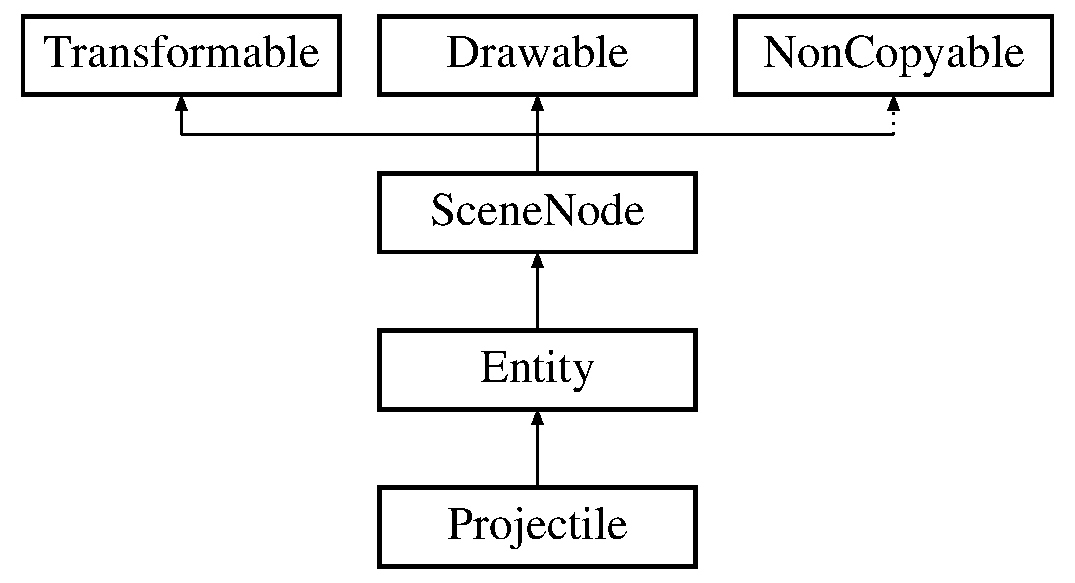
\includegraphics[height=4.000000cm]{class_projectile}
\end{center}
\end{figure}
\subsection*{Public Types}
\begin{DoxyCompactItemize}
\item 
\hypertarget{class_projectile_ae0d6ce4b663618b4105d2f3a483ff2eb}{}enum {\bfseries Type} \{ {\bfseries Allied\+Bullet}, 
{\bfseries Enemy\+Bullet}, 
{\bfseries Missile}, 
{\bfseries Type\+Count}
 \}\label{class_projectile_ae0d6ce4b663618b4105d2f3a483ff2eb}

\end{DoxyCompactItemize}
\subsection*{Public Member Functions}
\begin{DoxyCompactItemize}
\item 
\hypertarget{class_projectile_a3cc3cae5a10d2ba896788e48d2decca8}{}{\bfseries Projectile} (Type type, const \hyperlink{class_resource_holder}{Texture\+Holder} \&textures)\label{class_projectile_a3cc3cae5a10d2ba896788e48d2decca8}

\item 
\hypertarget{class_projectile_ab85ee596545164953d19763d92c2f28c}{}virtual unsigned int {\bfseries get\+Category} () const \label{class_projectile_ab85ee596545164953d19763d92c2f28c}

\item 
\hypertarget{class_projectile_a314fb24ac002d5674f81a6857237f77e}{}virtual sf\+::\+Float\+Rect {\bfseries get\+Bounding\+Rect} () const \label{class_projectile_a314fb24ac002d5674f81a6857237f77e}

\item 
\hypertarget{class_projectile_a1af562c4a58c674243a1422bec2afe91}{}float {\bfseries get\+Max\+Speed} () const \label{class_projectile_a1af562c4a58c674243a1422bec2afe91}

\item 
\hypertarget{class_projectile_a583638375c8772c196b59c1be1667a29}{}int {\bfseries get\+Damage} () const \label{class_projectile_a583638375c8772c196b59c1be1667a29}

\end{DoxyCompactItemize}
\subsection*{Additional Inherited Members}


The documentation for this class was generated from the following file\+:\begin{DoxyCompactItemize}
\item 
Include/\+Tanks/Projectile.\+hpp\end{DoxyCompactItemize}

\hypertarget{struct_projectile_data}{}\section{Projectile\+Data Struct Reference}
\label{struct_projectile_data}\index{Projectile\+Data@{Projectile\+Data}}
\subsection*{Public Attributes}
\begin{DoxyCompactItemize}
\item 
\hypertarget{struct_projectile_data_add13e5536e407fa142dc8dc1dea3959b}{}int {\bfseries damage}\label{struct_projectile_data_add13e5536e407fa142dc8dc1dea3959b}

\item 
\hypertarget{struct_projectile_data_ad5203e5d2fccba6c543de57d1e9070d5}{}float {\bfseries speed}\label{struct_projectile_data_ad5203e5d2fccba6c543de57d1e9070d5}

\item 
\hypertarget{struct_projectile_data_af72f694e0c4ef9fa6e034167a32592f9}{}Textures\+::\+I\+D {\bfseries texture}\label{struct_projectile_data_af72f694e0c4ef9fa6e034167a32592f9}

\end{DoxyCompactItemize}


The documentation for this struct was generated from the following file\+:\begin{DoxyCompactItemize}
\item 
Include/\+Tanks/Data\+Tables.\+hpp\end{DoxyCompactItemize}

\hypertarget{class_quadtree}{}\section{Quadtree Class Reference}
\label{class_quadtree}\index{Quadtree@{Quadtree}}
Inheritance diagram for Quadtree\+:\begin{figure}[H]
\begin{center}
\leavevmode
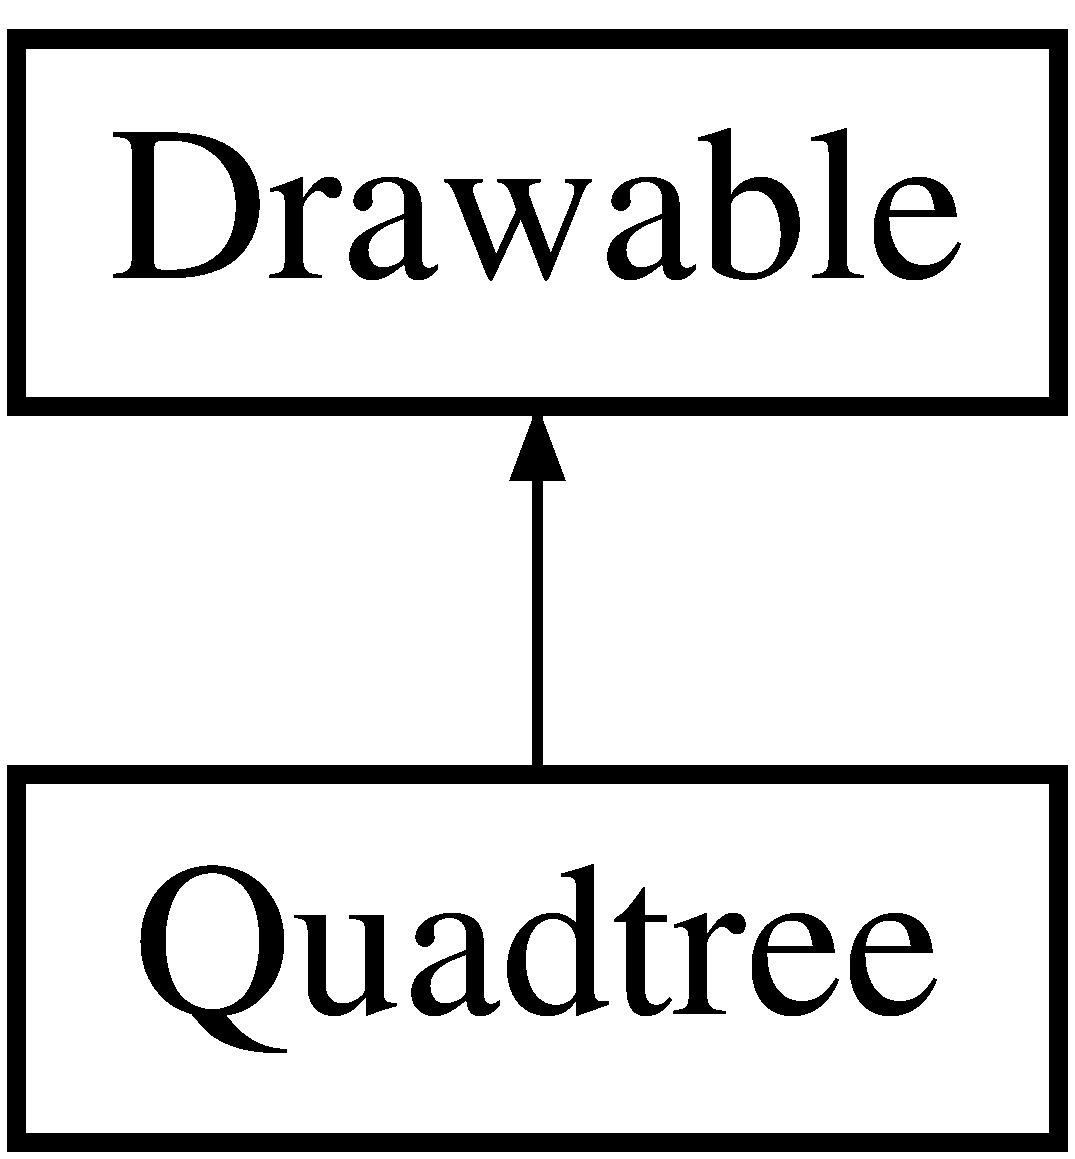
\includegraphics[height=2.000000cm]{class_quadtree}
\end{center}
\end{figure}
\subsection*{Public Member Functions}
\begin{DoxyCompactItemize}
\item 
\hypertarget{class_quadtree_a5c7b5645185e1994f6f8ae25eac9cbdd}{}{\bfseries Quadtree} (int level, sf\+::\+Float\+Rect bounds)\label{class_quadtree_a5c7b5645185e1994f6f8ae25eac9cbdd}

\item 
\hypertarget{class_quadtree_ab2b40ef82fa81688886c8f38bf7846d3}{}void {\bfseries clear} ()\label{class_quadtree_ab2b40ef82fa81688886c8f38bf7846d3}

\item 
\hypertarget{class_quadtree_a496a472afe2ebe39478ab089d4a3526a}{}void {\bfseries split} ()\label{class_quadtree_a496a472afe2ebe39478ab089d4a3526a}

\item 
\hypertarget{class_quadtree_a823eb501b292b4cce84fc5e779890027}{}int {\bfseries get\+Index} (const \hyperlink{class_scene_node}{Scene\+Node} \&scene\+Node) const \label{class_quadtree_a823eb501b292b4cce84fc5e779890027}

\item 
\hypertarget{class_quadtree_a7559d12bb7cb05c6e5c8ddddcbc1ec03}{}void {\bfseries insert} (\hyperlink{class_scene_node}{Scene\+Node} \&scene\+Node)\label{class_quadtree_a7559d12bb7cb05c6e5c8ddddcbc1ec03}

\item 
\hypertarget{class_quadtree_af1712ccec2952bfaf379c854b798eb47}{}std\+::vector$<$ \hyperlink{class_scene_node}{Scene\+Node} $\ast$ $>$ {\bfseries retrieve} (const \hyperlink{class_scene_node}{Scene\+Node} \&scene\+Node) const \label{class_quadtree_af1712ccec2952bfaf379c854b798eb47}

\item 
\hypertarget{class_quadtree_ad3956dc1f458ecd92be053465453dd57}{}sf\+::\+Float\+Rect {\bfseries get\+Bounds} () const \label{class_quadtree_ad3956dc1f458ecd92be053465453dd57}

\item 
\hypertarget{class_quadtree_a29c7e64da9ebbbf3c093c6d437e2f8e4}{}void {\bfseries set\+Bounds} (const sf\+::\+Float\+Rect \&rect)\label{class_quadtree_a29c7e64da9ebbbf3c093c6d437e2f8e4}

\item 
\hypertarget{class_quadtree_ad94ee55aa6e1d48aa3ab4958443d0b2f}{}virtual void {\bfseries draw} (sf\+::\+Render\+Target \&target, sf\+::\+Render\+States states) const \label{class_quadtree_ad94ee55aa6e1d48aa3ab4958443d0b2f}

\end{DoxyCompactItemize}


The documentation for this class was generated from the following file\+:\begin{DoxyCompactItemize}
\item 
Include/\+Tanks/Quadtree.\+hpp\end{DoxyCompactItemize}

\hypertarget{class_resource_holder}{}\section{Resource\+Holder$<$ Resource, Identifier $>$ Class Template Reference}
\label{class_resource_holder}\index{Resource\+Holder$<$ Resource, Identifier $>$@{Resource\+Holder$<$ Resource, Identifier $>$}}
\subsection*{Public Member Functions}
\begin{DoxyCompactItemize}
\item 
\hypertarget{class_resource_holder_accb6a2b6bd2da503ddfd57b5c0028a16}{}void {\bfseries load} (Identifier id, const std\+::string \&filename)\label{class_resource_holder_accb6a2b6bd2da503ddfd57b5c0028a16}

\item 
\hypertarget{class_resource_holder_ae83a7a88b2b2a74b6143796eb4452110}{}{\footnotesize template$<$typename Parameter $>$ }\\void {\bfseries load} (Identifier id, const std\+::string \&filename, const Parameter \&second\+Param)\label{class_resource_holder_ae83a7a88b2b2a74b6143796eb4452110}

\item 
\hypertarget{class_resource_holder_a236988b27b59d66e39e38e556de2a064}{}Resource \& {\bfseries get} (Identifier id)\label{class_resource_holder_a236988b27b59d66e39e38e556de2a064}

\item 
\hypertarget{class_resource_holder_a3de78ac3453a9eff9979da463f0f51e1}{}const Resource \& {\bfseries get} (Identifier id) const \label{class_resource_holder_a3de78ac3453a9eff9979da463f0f51e1}

\end{DoxyCompactItemize}


The documentation for this class was generated from the following file\+:\begin{DoxyCompactItemize}
\item 
Include/\+Tanks/Resource\+Holder.\+hpp\end{DoxyCompactItemize}

\hypertarget{class_scene_node}{}\section{Scene\+Node Class Reference}
\label{class_scene_node}\index{Scene\+Node@{Scene\+Node}}
Inheritance diagram for Scene\+Node\+:\begin{figure}[H]
\begin{center}
\leavevmode
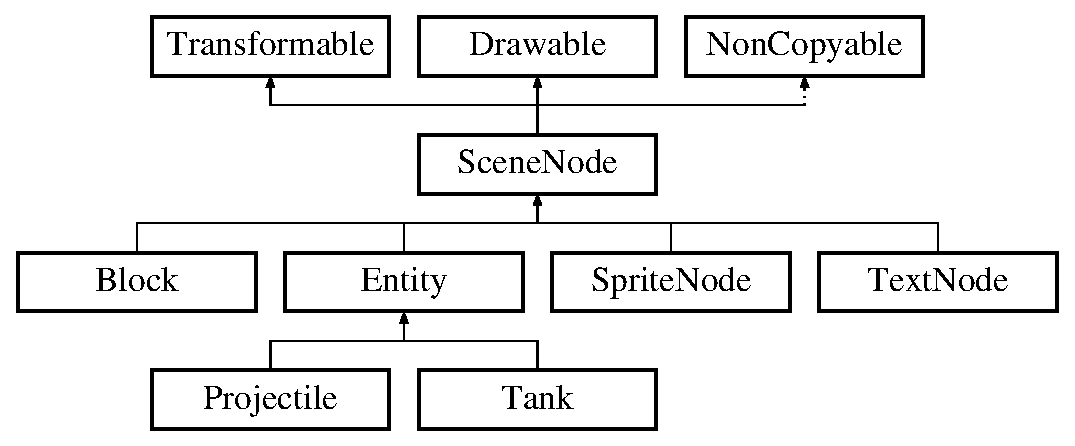
\includegraphics[height=4.000000cm]{class_scene_node}
\end{center}
\end{figure}
\subsection*{Public Types}
\begin{DoxyCompactItemize}
\item 
\hypertarget{class_scene_node_aaf5c9ad8475874b51b70e400822f2e9a}{}typedef std\+::unique\+\_\+ptr$<$ \hyperlink{class_scene_node}{Scene\+Node} $>$ {\bfseries Ptr}\label{class_scene_node_aaf5c9ad8475874b51b70e400822f2e9a}

\item 
\hypertarget{class_scene_node_a366efca54698fa3f6eaf80b41e7ff4df}{}typedef std\+::pair$<$ \hyperlink{class_scene_node}{Scene\+Node} $\ast$, \hyperlink{class_scene_node}{Scene\+Node} $\ast$ $>$ {\bfseries Pair}\label{class_scene_node_a366efca54698fa3f6eaf80b41e7ff4df}

\end{DoxyCompactItemize}
\subsection*{Public Member Functions}
\begin{DoxyCompactItemize}
\item 
\hypertarget{class_scene_node_ae6066cf0e6c0bddbc06e6d09bac918e9}{}{\bfseries Scene\+Node} (Category\+::\+Type category=Category\+::\+None)\label{class_scene_node_ae6066cf0e6c0bddbc06e6d09bac918e9}

\item 
\hypertarget{class_scene_node_acdfa2c2ba28bce076c886eaba2d9e650}{}void {\bfseries attach\+Child} (Ptr child)\label{class_scene_node_acdfa2c2ba28bce076c886eaba2d9e650}

\item 
\hypertarget{class_scene_node_ae7bfc285268dcbda5d406e0185f63262}{}Ptr {\bfseries detach\+Child} (const \hyperlink{class_scene_node}{Scene\+Node} \&node)\label{class_scene_node_ae7bfc285268dcbda5d406e0185f63262}

\item 
\hypertarget{class_scene_node_a5494c3a380d7ea5ae7148122c4255400}{}void {\bfseries update} (sf\+::\+Time dt, \hyperlink{class_command_queue}{Command\+Queue} \&commands)\label{class_scene_node_a5494c3a380d7ea5ae7148122c4255400}

\item 
\hypertarget{class_scene_node_a410150636d06294c7a9e238d8c4f07b5}{}sf\+::\+Vector2f {\bfseries get\+World\+Position} () const \label{class_scene_node_a410150636d06294c7a9e238d8c4f07b5}

\item 
\hypertarget{class_scene_node_a88be3d3c93c80ee4a7ba25024d2414ec}{}sf\+::\+Transform {\bfseries get\+World\+Transform} () const \label{class_scene_node_a88be3d3c93c80ee4a7ba25024d2414ec}

\item 
\hypertarget{class_scene_node_afcb3176686c13d320ca0bfb0c22bbd4f}{}void {\bfseries check\+Node\+Collision} (\hyperlink{class_scene_node}{Scene\+Node} \&node, std\+::set$<$ Pair $>$ \&collision\+Pairs)\label{class_scene_node_afcb3176686c13d320ca0bfb0c22bbd4f}

\item 
\hypertarget{class_scene_node_adc84f9ef6a872340ff5489b54d9bf626}{}void {\bfseries check\+Scene\+Collision} (\hyperlink{class_scene_node}{Scene\+Node} \&scene\+Graph, std\+::set$<$ Pair $>$ \&collision\+Pairs)\label{class_scene_node_adc84f9ef6a872340ff5489b54d9bf626}

\item 
\hypertarget{class_scene_node_a3b15fb3228666c1e125c051172d16dd6}{}void {\bfseries check\+Collisions\+In\+Quadtree} (const \hyperlink{class_quadtree}{Quadtree} \&quadtree, std\+::set$<$ Pair $>$ \&collision\+Pairs)\label{class_scene_node_a3b15fb3228666c1e125c051172d16dd6}

\item 
\hypertarget{class_scene_node_a4ab07dfa68f4094e2e9152b6f4869794}{}void {\bfseries remove\+Wrecks} ()\label{class_scene_node_a4ab07dfa68f4094e2e9152b6f4869794}

\item 
\hypertarget{class_scene_node_af6f126fe8727414a0c967f84f9754968}{}void {\bfseries on\+Command} (const \hyperlink{struct_command}{Command} \&command, sf\+::\+Time dt)\label{class_scene_node_af6f126fe8727414a0c967f84f9754968}

\item 
\hypertarget{class_scene_node_a72984f6cf6427652da17e2e7dc9edb84}{}virtual unsigned int {\bfseries get\+Category} () const \label{class_scene_node_a72984f6cf6427652da17e2e7dc9edb84}

\item 
\hypertarget{class_scene_node_a6bcdee1ae95e703567854b832de3cbd2}{}virtual sf\+::\+Float\+Rect {\bfseries get\+Bounding\+Rect} () const \label{class_scene_node_a6bcdee1ae95e703567854b832de3cbd2}

\item 
\hypertarget{class_scene_node_a7a3cd583ac2252d19f12f6ab80df8a4a}{}virtual bool {\bfseries is\+Marked\+For\+Removal} () const \label{class_scene_node_a7a3cd583ac2252d19f12f6ab80df8a4a}

\item 
\hypertarget{class_scene_node_aa5ab9eec31659d093d4aa48d69573de9}{}virtual bool {\bfseries is\+Destroyed} () const \label{class_scene_node_aa5ab9eec31659d093d4aa48d69573de9}

\item 
\hypertarget{class_scene_node_a3204ee8a2551705287b06efc4590909e}{}void {\bfseries insert\+Into\+Quadtree} (\hyperlink{class_quadtree}{Quadtree} \&quadtree)\label{class_scene_node_a3204ee8a2551705287b06efc4590909e}

\end{DoxyCompactItemize}


The documentation for this class was generated from the following file\+:\begin{DoxyCompactItemize}
\item 
Include/\+Tanks/Scene\+Node.\+hpp\end{DoxyCompactItemize}

\hypertarget{class_settings_state}{}\section{Settings\+State Class Reference}
\label{class_settings_state}\index{Settings\+State@{Settings\+State}}
Inheritance diagram for Settings\+State\+:\begin{figure}[H]
\begin{center}
\leavevmode
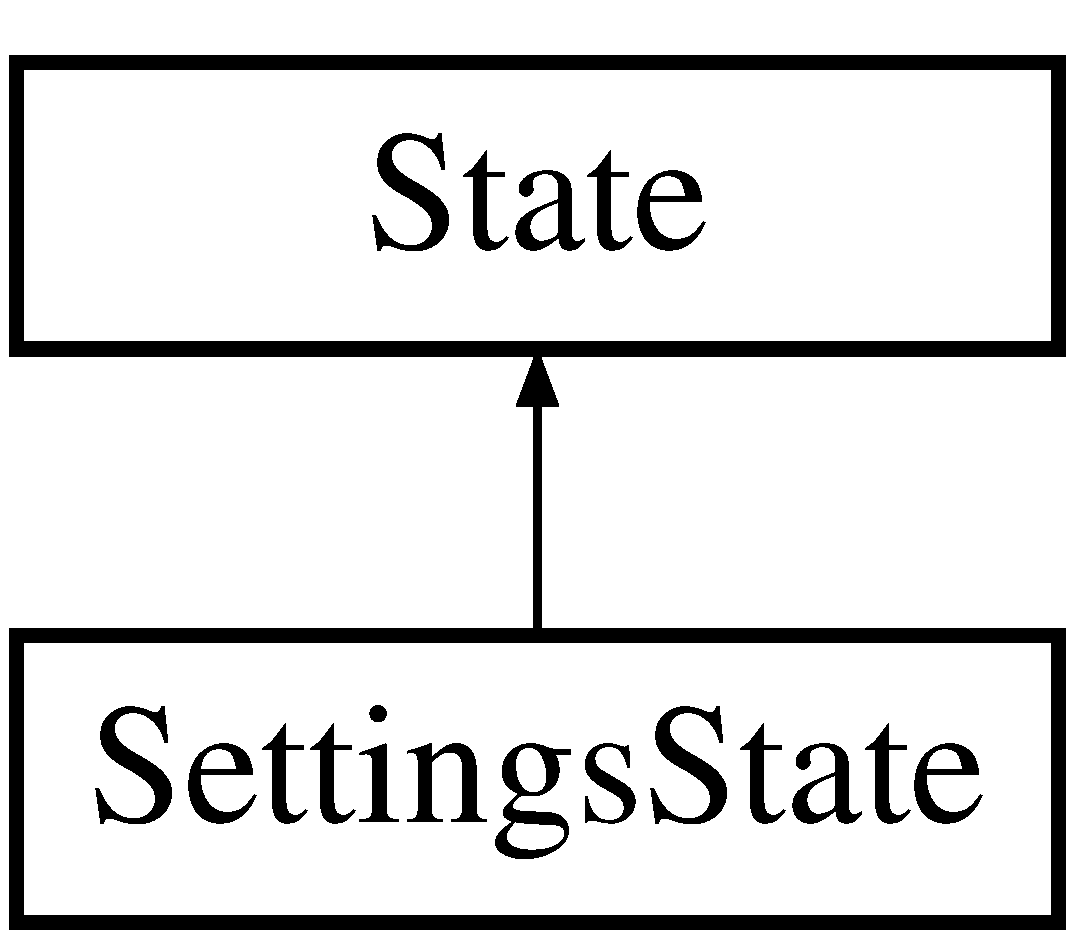
\includegraphics[height=2.000000cm]{class_settings_state}
\end{center}
\end{figure}
\subsection*{Public Member Functions}
\begin{DoxyCompactItemize}
\item 
\hypertarget{class_settings_state_a949344118b93b89df8426ff84bac3d3b}{}{\bfseries Settings\+State} (\hyperlink{class_state_stack}{State\+Stack} \&stack, \hyperlink{struct_state_1_1_context}{Context} context)\label{class_settings_state_a949344118b93b89df8426ff84bac3d3b}

\item 
\hypertarget{class_settings_state_a4398844b0b4a5945159d1396759dc870}{}virtual void {\bfseries draw} ()\label{class_settings_state_a4398844b0b4a5945159d1396759dc870}

\item 
\hypertarget{class_settings_state_a2514872c685a2da59ca903aa82fa22a9}{}virtual bool {\bfseries update} (sf\+::\+Time dt)\label{class_settings_state_a2514872c685a2da59ca903aa82fa22a9}

\item 
\hypertarget{class_settings_state_a4cc7a66d730634afa6fcefff96f82268}{}virtual bool {\bfseries handle\+Event} (const sf\+::\+Event \&event)\label{class_settings_state_a4cc7a66d730634afa6fcefff96f82268}

\end{DoxyCompactItemize}
\subsection*{Additional Inherited Members}


The documentation for this class was generated from the following file\+:\begin{DoxyCompactItemize}
\item 
Include/\+Tanks/Settings\+State.\+hpp\end{DoxyCompactItemize}

\hypertarget{class_sprite_node}{}\section{Sprite\+Node Class Reference}
\label{class_sprite_node}\index{Sprite\+Node@{Sprite\+Node}}
Inheritance diagram for Sprite\+Node\+:\begin{figure}[H]
\begin{center}
\leavevmode
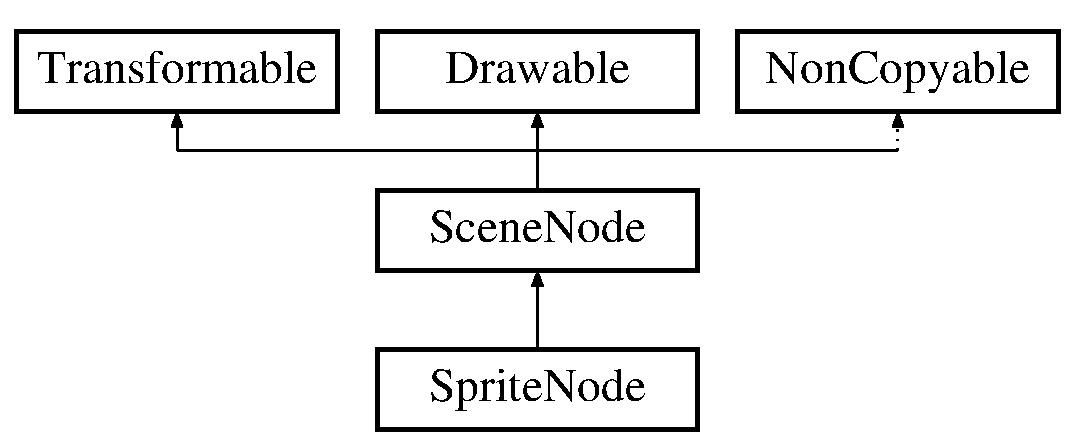
\includegraphics[height=3.000000cm]{class_sprite_node}
\end{center}
\end{figure}
\subsection*{Public Member Functions}
\begin{DoxyCompactItemize}
\item 
\hypertarget{class_sprite_node_ad72b769f4c57e5d77a8d6ba223f487b0}{}{\bfseries Sprite\+Node} (const sf\+::\+Texture \&texture)\label{class_sprite_node_ad72b769f4c57e5d77a8d6ba223f487b0}

\item 
\hypertarget{class_sprite_node_ac12927969dcfd6f02da372e7e22c2af1}{}{\bfseries Sprite\+Node} (const sf\+::\+Texture \&texture, const sf\+::\+Int\+Rect \&texture\+Rect)\label{class_sprite_node_ac12927969dcfd6f02da372e7e22c2af1}

\end{DoxyCompactItemize}
\subsection*{Additional Inherited Members}


The documentation for this class was generated from the following file\+:\begin{DoxyCompactItemize}
\item 
Include/\+Tanks/Sprite\+Node.\+hpp\end{DoxyCompactItemize}

\hypertarget{class_state}{}\section{State Class Reference}
\label{class_state}\index{State@{State}}
Inheritance diagram for State\+:\begin{figure}[H]
\begin{center}
\leavevmode
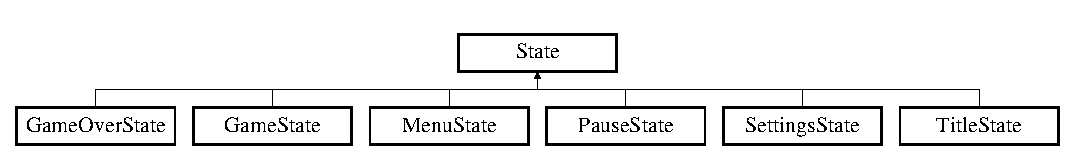
\includegraphics[height=1.712538cm]{class_state}
\end{center}
\end{figure}
\subsection*{Classes}
\begin{DoxyCompactItemize}
\item 
struct \hyperlink{struct_state_1_1_context}{Context}
\end{DoxyCompactItemize}
\subsection*{Public Types}
\begin{DoxyCompactItemize}
\item 
\hypertarget{class_state_a71d9930be1a58be7f711e245b7965d48}{}typedef std\+::unique\+\_\+ptr$<$ \hyperlink{class_state}{State} $>$ {\bfseries Ptr}\label{class_state_a71d9930be1a58be7f711e245b7965d48}

\end{DoxyCompactItemize}
\subsection*{Public Member Functions}
\begin{DoxyCompactItemize}
\item 
\hypertarget{class_state_afede488ff3c1b264bbd07f8aeead84a7}{}{\bfseries State} (\hyperlink{class_state_stack}{State\+Stack} \&stack, \hyperlink{struct_state_1_1_context}{Context} context)\label{class_state_afede488ff3c1b264bbd07f8aeead84a7}

\item 
\hypertarget{class_state_ae261605bc40b7e3959ce5df5457e4942}{}virtual void {\bfseries draw} ()=0\label{class_state_ae261605bc40b7e3959ce5df5457e4942}

\item 
\hypertarget{class_state_acd5926bc7a373edff9e57f3ffe94ca13}{}virtual bool {\bfseries update} (sf\+::\+Time dt)=0\label{class_state_acd5926bc7a373edff9e57f3ffe94ca13}

\item 
\hypertarget{class_state_a19965f83460b248c42952aac8d001206}{}virtual bool {\bfseries handle\+Event} (const sf\+::\+Event \&event)=0\label{class_state_a19965f83460b248c42952aac8d001206}

\end{DoxyCompactItemize}
\subsection*{Protected Member Functions}
\begin{DoxyCompactItemize}
\item 
\hypertarget{class_state_a6763de833ceb9c23df45aff163a4a1cd}{}void {\bfseries request\+Stack\+Push} (States\+::\+I\+D state\+I\+D)\label{class_state_a6763de833ceb9c23df45aff163a4a1cd}

\item 
\hypertarget{class_state_aa418660892d6161772c907bd8d70f910}{}void {\bfseries request\+Stack\+Pop} ()\label{class_state_aa418660892d6161772c907bd8d70f910}

\item 
\hypertarget{class_state_a4b602bed9bf0179ee5f6748fce340ae6}{}void {\bfseries request\+State\+Clear} ()\label{class_state_a4b602bed9bf0179ee5f6748fce340ae6}

\item 
\hypertarget{class_state_aec041e226f59f134902ca8671c02788c}{}\hyperlink{struct_state_1_1_context}{Context} {\bfseries get\+Context} () const \label{class_state_aec041e226f59f134902ca8671c02788c}

\end{DoxyCompactItemize}


The documentation for this class was generated from the following file\+:\begin{DoxyCompactItemize}
\item 
Include/\+Tanks/State.\+hpp\end{DoxyCompactItemize}

\hypertarget{class_state_stack}{}\section{State\+Stack Class Reference}
\label{class_state_stack}\index{State\+Stack@{State\+Stack}}
Inheritance diagram for State\+Stack\+:\begin{figure}[H]
\begin{center}
\leavevmode
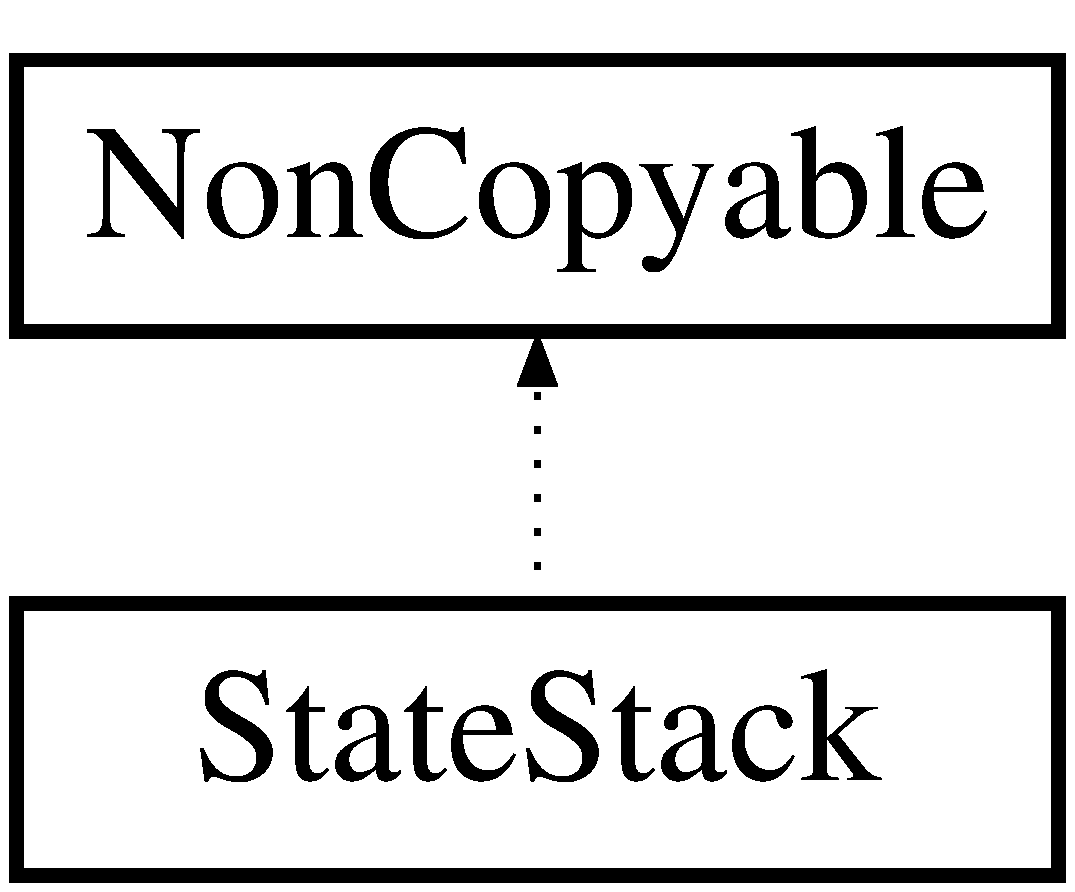
\includegraphics[height=2.000000cm]{class_state_stack}
\end{center}
\end{figure}
\subsection*{Public Types}
\begin{DoxyCompactItemize}
\item 
\hypertarget{class_state_stack_af804142a55cd477767353e0abbcc218c}{}enum {\bfseries Action} \{ {\bfseries Push}, 
{\bfseries Pop}, 
{\bfseries Clear}
 \}\label{class_state_stack_af804142a55cd477767353e0abbcc218c}

\end{DoxyCompactItemize}
\subsection*{Public Member Functions}
\begin{DoxyCompactItemize}
\item 
\hypertarget{class_state_stack_a365f29afd04a9370f6638cbe3b4ff92a}{}{\bfseries State\+Stack} (\hyperlink{struct_state_1_1_context}{State\+::\+Context} context)\label{class_state_stack_a365f29afd04a9370f6638cbe3b4ff92a}

\item 
\hypertarget{class_state_stack_a9d64daa479c2cccad6f2ede77741a352}{}{\footnotesize template$<$typename T $>$ }\\void {\bfseries register\+State} (States\+::\+I\+D state\+I\+D)\label{class_state_stack_a9d64daa479c2cccad6f2ede77741a352}

\item 
\hypertarget{class_state_stack_ae90af9f56ce7774d47d0407e2680c27d}{}void {\bfseries update} (sf\+::\+Time dt)\label{class_state_stack_ae90af9f56ce7774d47d0407e2680c27d}

\item 
\hypertarget{class_state_stack_a0990b973b2a0bdf8fad2f326e564931a}{}void {\bfseries draw} ()\label{class_state_stack_a0990b973b2a0bdf8fad2f326e564931a}

\item 
\hypertarget{class_state_stack_a70d3ffad9da499b8356789115f3e2acf}{}void {\bfseries handle\+Event} (const sf\+::\+Event \&event)\label{class_state_stack_a70d3ffad9da499b8356789115f3e2acf}

\item 
\hypertarget{class_state_stack_a80ed85f0fc13039e6f4c7dfef19e608f}{}void {\bfseries push\+State} (States\+::\+I\+D state\+I\+D)\label{class_state_stack_a80ed85f0fc13039e6f4c7dfef19e608f}

\item 
\hypertarget{class_state_stack_a7e050a57b798295c2344f1318765b5ee}{}void {\bfseries pop\+State} ()\label{class_state_stack_a7e050a57b798295c2344f1318765b5ee}

\item 
\hypertarget{class_state_stack_a49f0703d4037c3bf63494e64cb09898d}{}void {\bfseries clear\+States} ()\label{class_state_stack_a49f0703d4037c3bf63494e64cb09898d}

\item 
\hypertarget{class_state_stack_a63a73898d24eb0a68cac0215a9fda4fc}{}bool {\bfseries is\+Empty} () const \label{class_state_stack_a63a73898d24eb0a68cac0215a9fda4fc}

\end{DoxyCompactItemize}


The documentation for this class was generated from the following file\+:\begin{DoxyCompactItemize}
\item 
Include/\+Tanks/State\+Stack.\+hpp\end{DoxyCompactItemize}

\hypertarget{class_tank}{}\section{Tank Class Reference}
\label{class_tank}\index{Tank@{Tank}}
Inheritance diagram for Tank\+:\begin{figure}[H]
\begin{center}
\leavevmode
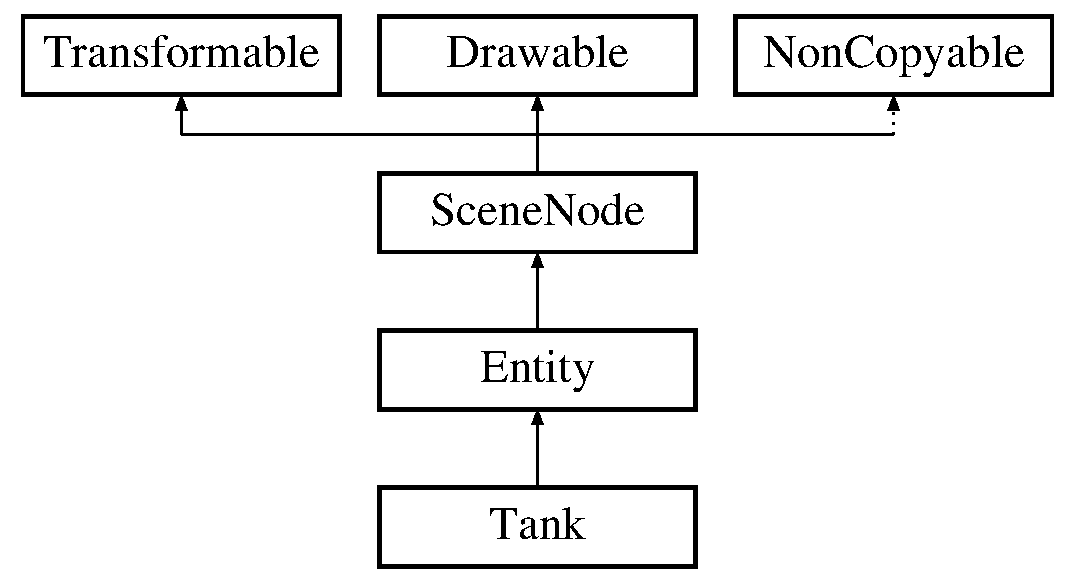
\includegraphics[height=4.000000cm]{class_tank}
\end{center}
\end{figure}
\subsection*{Public Types}
\begin{DoxyCompactItemize}
\item 
\hypertarget{class_tank_a9bb1855539f5e229bcdd517c127d34d9}{}enum {\bfseries Type} \{ \\*
{\bfseries Hero}, 
{\bfseries Dummy}, 
{\bfseries Hunting1}, 
{\bfseries Hunting2}, 
\\*
{\bfseries Guarding1}, 
{\bfseries Type\+Count}
 \}\label{class_tank_a9bb1855539f5e229bcdd517c127d34d9}

\end{DoxyCompactItemize}
\subsection*{Public Member Functions}
\begin{DoxyCompactItemize}
\item 
\hypertarget{class_tank_a416585727f18a9c471cb82a273036194}{}{\bfseries Tank} (Type type, const \hyperlink{class_resource_holder}{Texture\+Holder} \&textures, const \hyperlink{class_resource_holder}{Font\+Holder} \&fonts)\label{class_tank_a416585727f18a9c471cb82a273036194}

\item 
\hypertarget{class_tank_a5be180a933ca4e21206c1c283b7875f6}{}void {\bfseries set\+Rotation\+Offset} (float angle)\label{class_tank_a5be180a933ca4e21206c1c283b7875f6}

\item 
\hypertarget{class_tank_a3cc1280d4f77e41eed5832520e04a451}{}void {\bfseries rotate} (float offset)\label{class_tank_a3cc1280d4f77e41eed5832520e04a451}

\item 
\hypertarget{class_tank_a1e7aad0bafbebf4228f8268dc65828ad}{}float {\bfseries get\+Rotation\+Offset} () const \label{class_tank_a1e7aad0bafbebf4228f8268dc65828ad}

\item 
\hypertarget{class_tank_a2345439b017c3632bdfa3ab29b056669}{}virtual unsigned int {\bfseries get\+Category} () const \label{class_tank_a2345439b017c3632bdfa3ab29b056669}

\item 
\hypertarget{class_tank_a3b2728cc9d2385dccdc45a0c6160e5db}{}virtual sf\+::\+Float\+Rect {\bfseries get\+Bounding\+Rect} () const \label{class_tank_a3b2728cc9d2385dccdc45a0c6160e5db}

\item 
\hypertarget{class_tank_a9b1c6f05d8276c7335036575ddca2e8c}{}virtual bool {\bfseries is\+Marked\+For\+Removal} () const \label{class_tank_a9b1c6f05d8276c7335036575ddca2e8c}

\item 
\hypertarget{class_tank_ae280cab799bf1ebb08ea42648736dd1f}{}Type {\bfseries get\+Type} () const \label{class_tank_ae280cab799bf1ebb08ea42648736dd1f}

\item 
\hypertarget{class_tank_a9f48804a0a44929063b9ff9a1280e0b9}{}bool {\bfseries is\+Allied} () const \label{class_tank_a9f48804a0a44929063b9ff9a1280e0b9}

\item 
\hypertarget{class_tank_abb0f52ede672bcb8cdfa1dd4a340a91b}{}bool {\bfseries is\+Moving\+Towards\+Player} () const \label{class_tank_abb0f52ede672bcb8cdfa1dd4a340a91b}

\item 
\hypertarget{class_tank_a4efa3834dc7e18840c9d42a4958c9046}{}float {\bfseries get\+Max\+Movement\+Speed} () const \label{class_tank_a4efa3834dc7e18840c9d42a4958c9046}

\item 
\hypertarget{class_tank_ae40715b4f892f914eed657cca6a2e0ff}{}float {\bfseries get\+Max\+Rotation\+Speed} () const \label{class_tank_ae40715b4f892f914eed657cca6a2e0ff}

\item 
\hypertarget{class_tank_a037ffda79506d0f1392bc83d2edd0868}{}float {\bfseries get\+Travelled\+Distance} () const \label{class_tank_a037ffda79506d0f1392bc83d2edd0868}

\item 
\hypertarget{class_tank_a35208f172dbcc8b6f8e3638231f29e5a}{}void {\bfseries set\+Travelled\+Distance} (float distance)\label{class_tank_a35208f172dbcc8b6f8e3638231f29e5a}

\item 
\hypertarget{class_tank_adf1971fd4de92ac0ba9af0e4a6660659}{}float {\bfseries get\+Amount\+Rotated} () const \label{class_tank_adf1971fd4de92ac0ba9af0e4a6660659}

\item 
\hypertarget{class_tank_a8e12f38946222c9fba1bc60190e23b53}{}void {\bfseries set\+Amount\+Rotated} (float rotation)\label{class_tank_a8e12f38946222c9fba1bc60190e23b53}

\item 
\hypertarget{class_tank_aebe2d42e18e459979cbb5e9aeb6f6430}{}std\+::size\+\_\+t {\bfseries get\+Direction\+Index} () const \label{class_tank_aebe2d42e18e459979cbb5e9aeb6f6430}

\item 
\hypertarget{class_tank_ad943e5d63eedd0eaaf942b11dcf24209}{}void {\bfseries set\+Direction\+Index} (std\+::size\+\_\+t index)\label{class_tank_ad943e5d63eedd0eaaf942b11dcf24209}

\item 
\hypertarget{class_tank_af88a2851fda437eb921c7adc84bf793d}{}float {\bfseries get\+Guarding\+Path\+Length} () const \label{class_tank_af88a2851fda437eb921c7adc84bf793d}

\item 
\hypertarget{class_tank_ab3ebae5a6177b76003792b21421cd1a8}{}void {\bfseries set\+Guarding\+Path\+Length} (float length)\label{class_tank_ab3ebae5a6177b76003792b21421cd1a8}

\item 
\hypertarget{class_tank_aac61fd8574da62d0e862c5b3ce083a3e}{}float {\bfseries get\+Guarding\+Angle} () const \label{class_tank_aac61fd8574da62d0e862c5b3ce083a3e}

\item 
\hypertarget{class_tank_ad4557e537ce6d8cba6d713e11b18bfbb}{}void {\bfseries set\+Guarding\+Angle} (float angle)\label{class_tank_ad4557e537ce6d8cba6d713e11b18bfbb}

\item 
\hypertarget{class_tank_a41529cc679da94045b88b657b5c3e1e6}{}void {\bfseries add\+Collision\+With\+Tank} (sf\+::\+Float\+Rect intersection)\label{class_tank_a41529cc679da94045b88b657b5c3e1e6}

\item 
\hypertarget{class_tank_a58a1e84bf663aecc38280e19f243eab0}{}void {\bfseries add\+Collision\+With\+Block} (sf\+::\+Float\+Rect intersection)\label{class_tank_a58a1e84bf663aecc38280e19f243eab0}

\item 
\hypertarget{class_tank_aec8a4c16067540f772adacb6b2086c24}{}void {\bfseries fire} ()\label{class_tank_aec8a4c16067540f772adacb6b2086c24}

\end{DoxyCompactItemize}
\subsection*{Static Public Member Functions}
\begin{DoxyCompactItemize}
\item 
\hypertarget{class_tank_a2f556e7e3111622fa9cedf841a814e15}{}static int {\bfseries get\+Max\+Hitpoints} (Type type)\label{class_tank_a2f556e7e3111622fa9cedf841a814e15}

\end{DoxyCompactItemize}
\subsection*{Additional Inherited Members}


The documentation for this class was generated from the following file\+:\begin{DoxyCompactItemize}
\item 
Include/\+Tanks/Tank.\+hpp\end{DoxyCompactItemize}

\hypertarget{struct_tank_data}{}\section{Tank\+Data Struct Reference}
\label{struct_tank_data}\index{Tank\+Data@{Tank\+Data}}
\subsection*{Public Attributes}
\begin{DoxyCompactItemize}
\item 
\hypertarget{struct_tank_data_a6a326cc7ca48f045ed8510c21e01113f}{}int {\bfseries hitpoints}\label{struct_tank_data_a6a326cc7ca48f045ed8510c21e01113f}

\item 
\hypertarget{struct_tank_data_a169d885b98acaf324159e7c711cd6d58}{}float {\bfseries movement\+Speed}\label{struct_tank_data_a169d885b98acaf324159e7c711cd6d58}

\item 
\hypertarget{struct_tank_data_a4492fd65aa4dcf33a8d284586cff1234}{}float {\bfseries rotation\+Speed}\label{struct_tank_data_a4492fd65aa4dcf33a8d284586cff1234}

\item 
\hypertarget{struct_tank_data_a421107fc22c25356c1a2ecd617149cf3}{}Textures\+::\+I\+D {\bfseries texture}\label{struct_tank_data_a421107fc22c25356c1a2ecd617149cf3}

\item 
\hypertarget{struct_tank_data_a3d6bbc5040160e731f9a4cd9fd0ab4a3}{}sf\+::\+Time {\bfseries fire\+Interval}\label{struct_tank_data_a3d6bbc5040160e731f9a4cd9fd0ab4a3}

\item 
\hypertarget{struct_tank_data_a987dcffc34a24fa25b6eacf154f9e5b2}{}std\+::vector$<$ \hyperlink{struct_bullet_launch_data}{Bullet\+Launch\+Data} $>$ {\bfseries bullets}\label{struct_tank_data_a987dcffc34a24fa25b6eacf154f9e5b2}

\item 
\hypertarget{struct_tank_data_a25b90870f56325d4284b254f9ebb6587}{}std\+::vector$<$ \hyperlink{struct_direction}{Direction} $>$ {\bfseries directions}\label{struct_tank_data_a25b90870f56325d4284b254f9ebb6587}

\end{DoxyCompactItemize}


The documentation for this struct was generated from the following file\+:\begin{DoxyCompactItemize}
\item 
Include/\+Tanks/Data\+Tables.\+hpp\end{DoxyCompactItemize}

\hypertarget{class_text_node}{}\section{Text\+Node Class Reference}
\label{class_text_node}\index{Text\+Node@{Text\+Node}}
Inheritance diagram for Text\+Node\+:\begin{figure}[H]
\begin{center}
\leavevmode
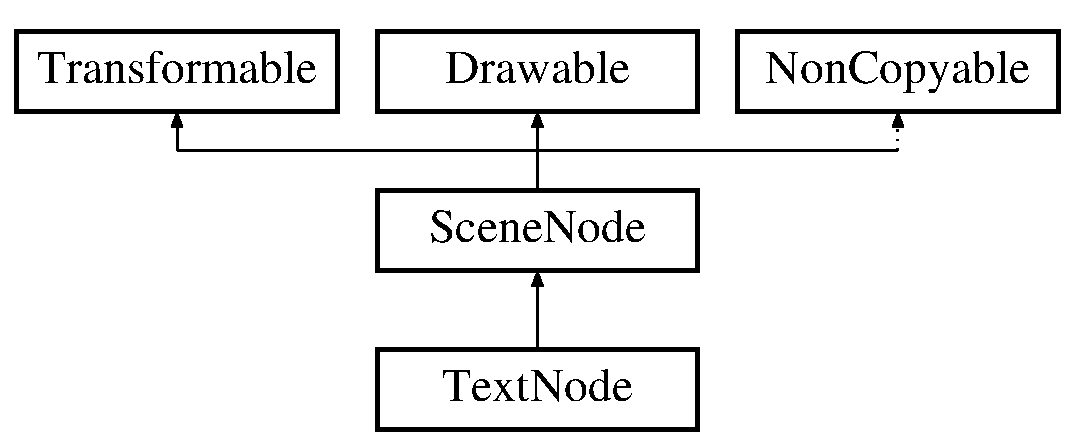
\includegraphics[height=3.000000cm]{class_text_node}
\end{center}
\end{figure}
\subsection*{Public Member Functions}
\begin{DoxyCompactItemize}
\item 
\hypertarget{class_text_node_a6ac9f0e37c705f4afdeb2c1888ca4084}{}{\bfseries Text\+Node} (const \hyperlink{class_resource_holder}{Font\+Holder} \&fonts, const std\+::string \&text)\label{class_text_node_a6ac9f0e37c705f4afdeb2c1888ca4084}

\item 
\hypertarget{class_text_node_a51c396c803287f43ee640c6b6421a212}{}void {\bfseries set\+String} (const std\+::string \&text)\label{class_text_node_a51c396c803287f43ee640c6b6421a212}

\end{DoxyCompactItemize}
\subsection*{Additional Inherited Members}


The documentation for this class was generated from the following file\+:\begin{DoxyCompactItemize}
\item 
Include/\+Tanks/Text\+Node.\+hpp\end{DoxyCompactItemize}

\hypertarget{class_title_state}{}\section{Title\+State Class Reference}
\label{class_title_state}\index{Title\+State@{Title\+State}}
Inheritance diagram for Title\+State\+:\begin{figure}[H]
\begin{center}
\leavevmode
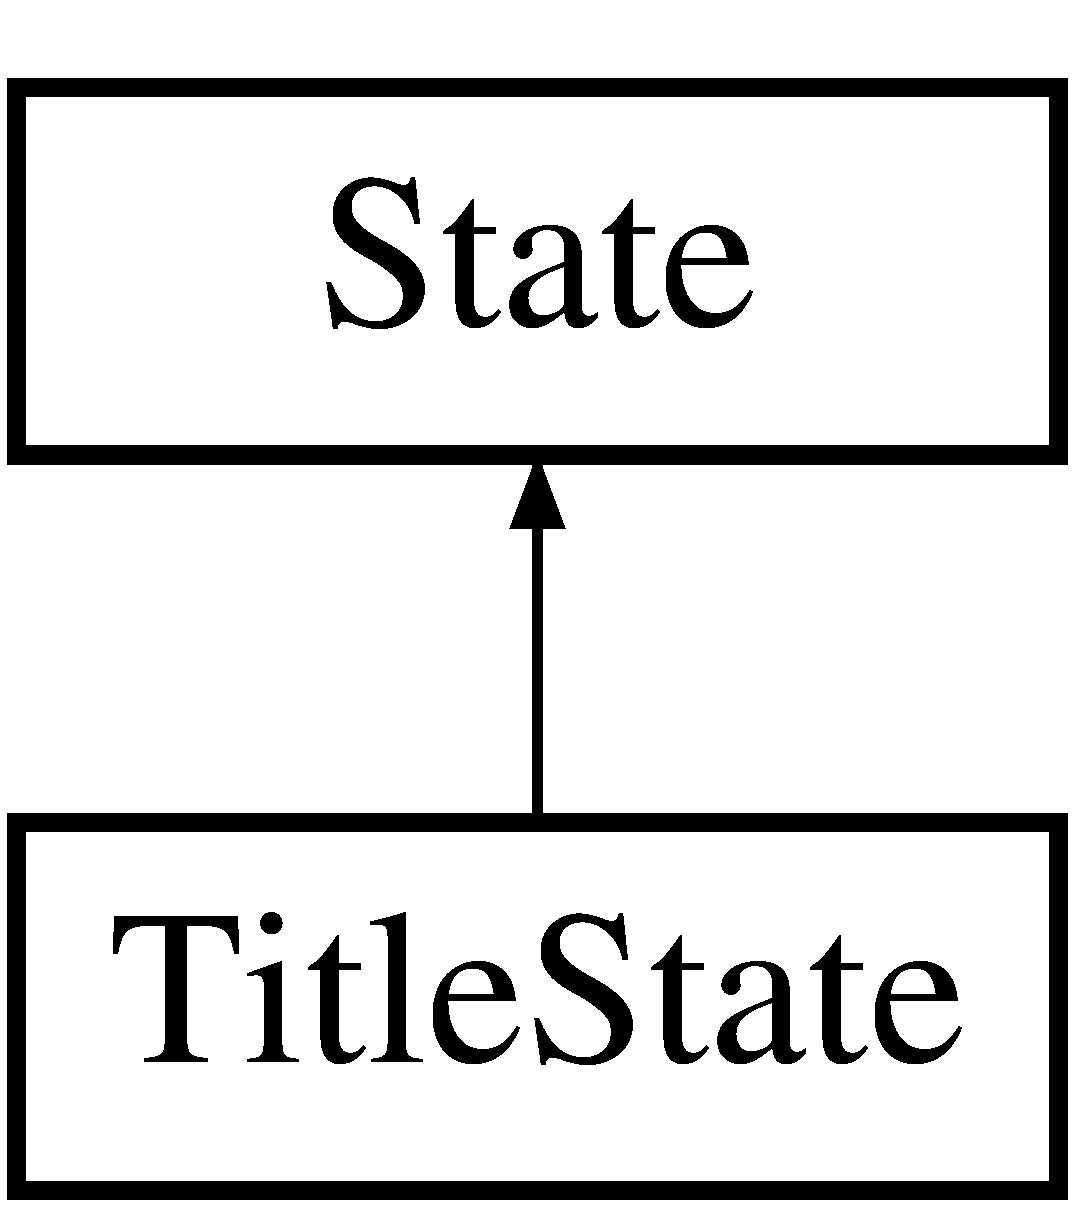
\includegraphics[height=2.000000cm]{class_title_state}
\end{center}
\end{figure}
\subsection*{Public Member Functions}
\begin{DoxyCompactItemize}
\item 
\hypertarget{class_title_state_a9fb6569d8ed77db85dcf8af2890c112c}{}{\bfseries Title\+State} (\hyperlink{class_state_stack}{State\+Stack} \&stack, \hyperlink{struct_state_1_1_context}{Context} context)\label{class_title_state_a9fb6569d8ed77db85dcf8af2890c112c}

\item 
\hypertarget{class_title_state_a0626f31f769d6f88eccc4880c153a0d2}{}virtual void {\bfseries draw} ()\label{class_title_state_a0626f31f769d6f88eccc4880c153a0d2}

\item 
\hypertarget{class_title_state_a722fcb2a30f05ea3821ea1ed4c841eec}{}virtual bool {\bfseries update} (sf\+::\+Time dt)\label{class_title_state_a722fcb2a30f05ea3821ea1ed4c841eec}

\item 
\hypertarget{class_title_state_af9e452529d3c3eeb4b8ee89cf8cb2ddf}{}virtual bool {\bfseries handle\+Event} (const sf\+::\+Event \&event)\label{class_title_state_af9e452529d3c3eeb4b8ee89cf8cb2ddf}

\end{DoxyCompactItemize}
\subsection*{Additional Inherited Members}


The documentation for this class was generated from the following file\+:\begin{DoxyCompactItemize}
\item 
Include/\+Tanks/Title\+State.\+hpp\end{DoxyCompactItemize}

\hypertarget{class_world}{}\section{World Class Reference}
\label{class_world}\index{World@{World}}
Inheritance diagram for World\+:\begin{figure}[H]
\begin{center}
\leavevmode
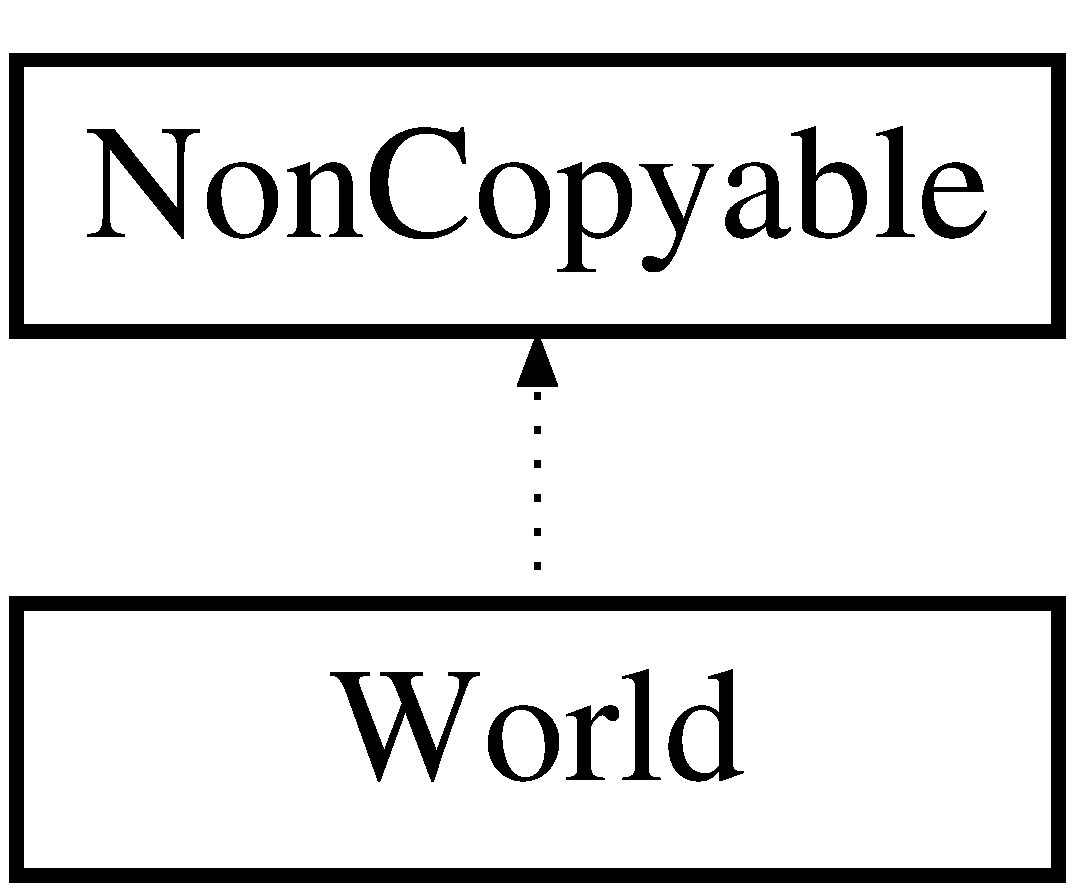
\includegraphics[height=2.000000cm]{class_world}
\end{center}
\end{figure}
\subsection*{Public Types}
\begin{DoxyCompactItemize}
\item 
\hypertarget{class_world_acb5af5bcc28f7190c116f49a6f4bd463}{}enum {\bfseries View\+Type} \{ {\bfseries Static}, 
{\bfseries Following}, 
{\bfseries Scrolling}
 \}\label{class_world_acb5af5bcc28f7190c116f49a6f4bd463}

\end{DoxyCompactItemize}
\subsection*{Public Member Functions}
\begin{DoxyCompactItemize}
\item 
\hypertarget{class_world_ad8c6499a2c10fb5ad5fe4e47ddbce5ed}{}{\bfseries World} (sf\+::\+Render\+Window \&window, \hyperlink{class_resource_holder}{Font\+Holder} \&fonts, \hyperlink{class_player}{Player} \&player)\label{class_world_ad8c6499a2c10fb5ad5fe4e47ddbce5ed}

\item 
\hypertarget{class_world_ac7b3a3923c95b812ec2d00d97c8cd56e}{}void {\bfseries update} (sf\+::\+Time dt)\label{class_world_ac7b3a3923c95b812ec2d00d97c8cd56e}

\item 
\hypertarget{class_world_ab51a17ccbb108616daacd0c34973dc8d}{}void {\bfseries draw} ()\label{class_world_ab51a17ccbb108616daacd0c34973dc8d}

\item 
\hypertarget{class_world_aa950faf89ee776af031062df93c0e5ff}{}\hyperlink{class_command_queue}{Command\+Queue} \& {\bfseries get\+Command\+Queue} ()\label{class_world_aa950faf89ee776af031062df93c0e5ff}

\item 
\hypertarget{class_world_a2a3d381e8e0bbe36dfa7203ff3aaefcb}{}bool {\bfseries has\+Alive\+Player} () const \label{class_world_a2a3d381e8e0bbe36dfa7203ff3aaefcb}

\item 
\hypertarget{class_world_a42191b670dcf2ddf8779b1fcce3f4e94}{}bool {\bfseries has\+Enemies} () const \label{class_world_a42191b670dcf2ddf8779b1fcce3f4e94}

\end{DoxyCompactItemize}


The documentation for this class was generated from the following file\+:\begin{DoxyCompactItemize}
\item 
Include/\+Tanks/World.\+hpp\end{DoxyCompactItemize}

%--- End generated contents ---

% Index
\backmatter
\newpage
\phantomsection
\clearemptydoublepage
\addcontentsline{toc}{chapter}{Index}
\printindex

\end{document}
